\chapter*{第八部分:学习、记忆、语言与认知}
\markboth{总论}{总论}


\begin{figure}[htbp]
	\centering
	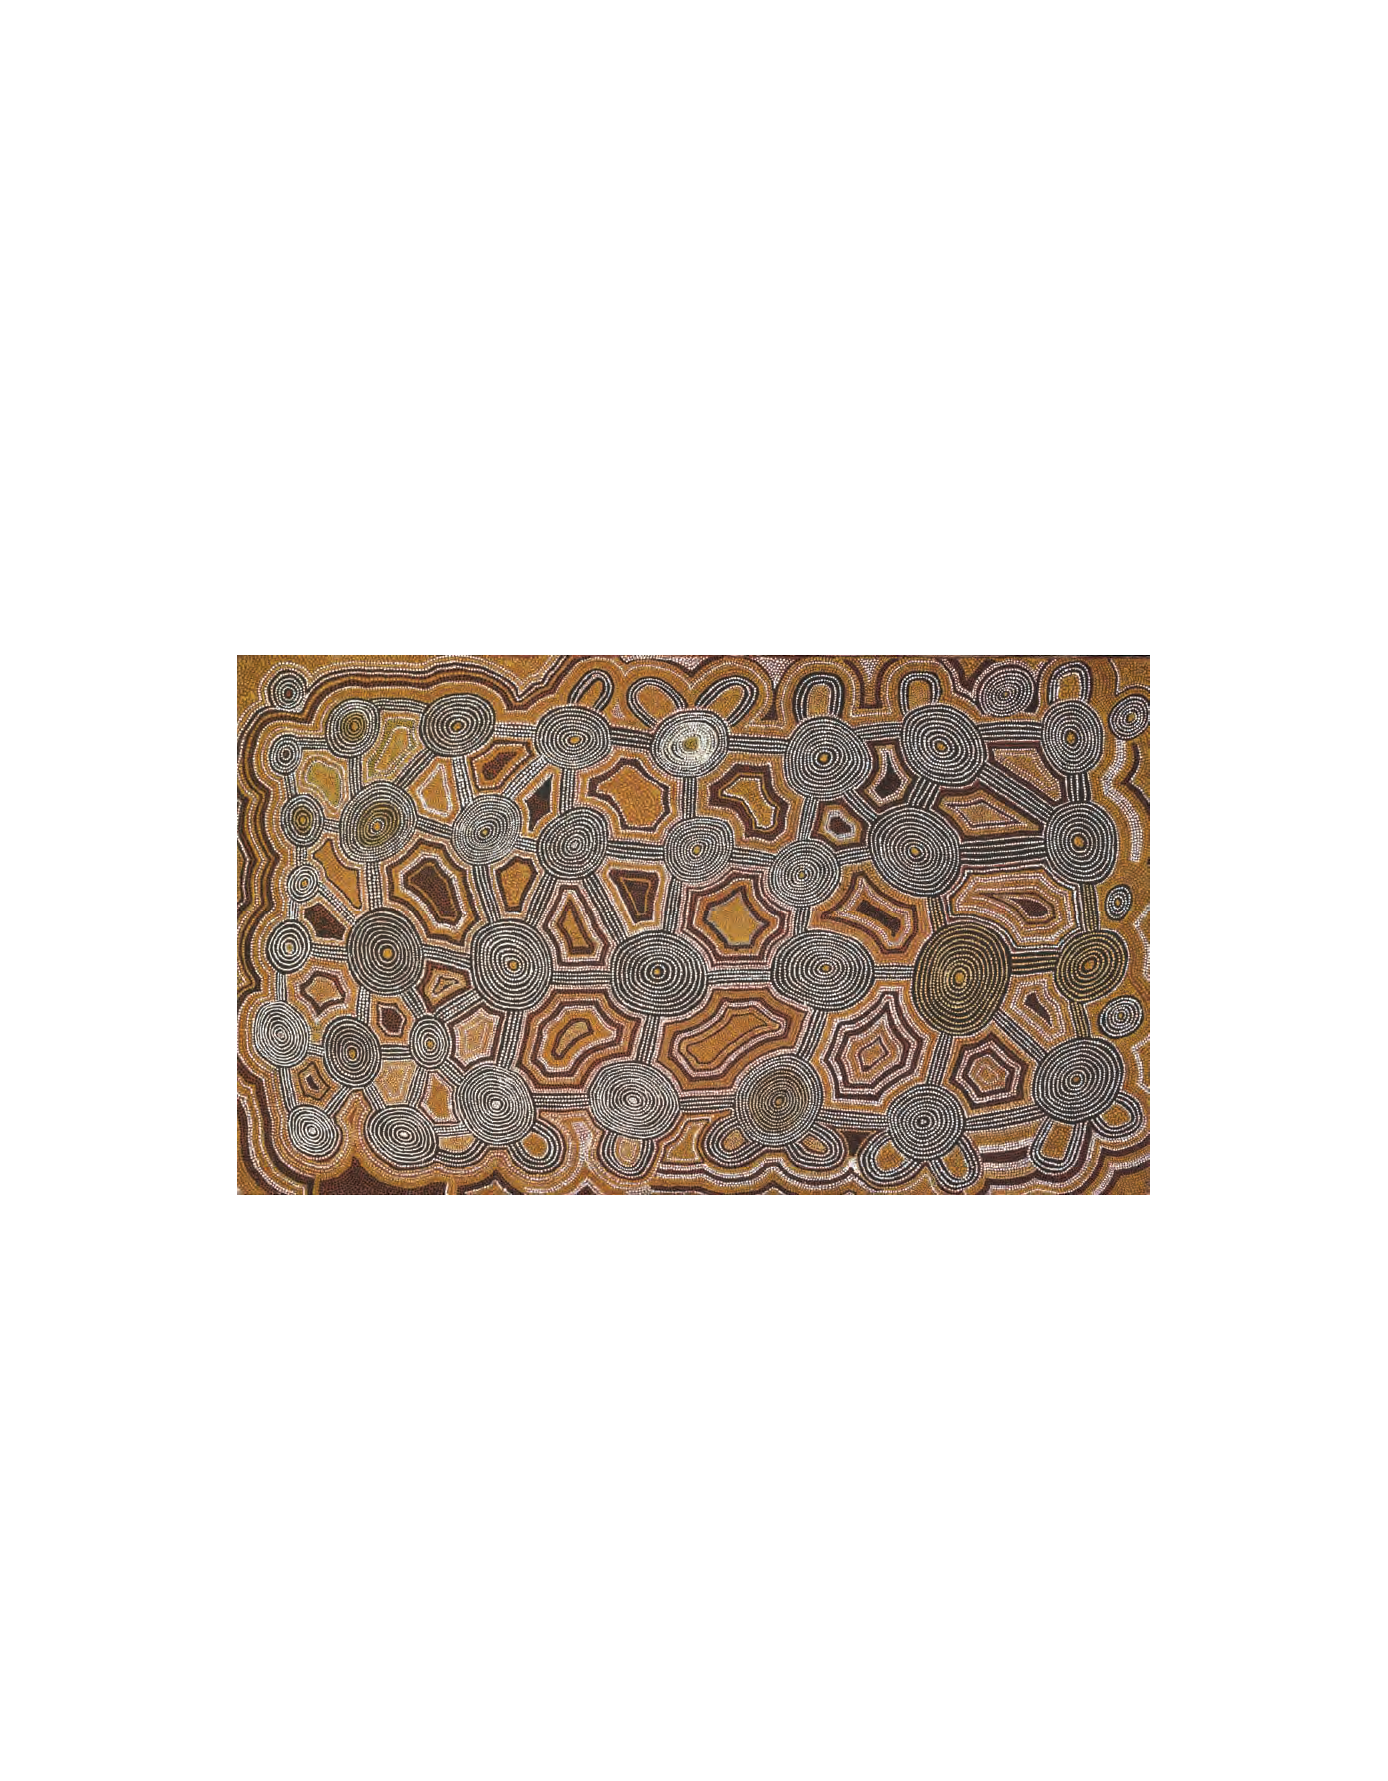
\includegraphics[width=1.0\linewidth]{chap52/fig_52_0}
	\caption{马拉宾丁亚的廷加里人和同修。
		在澳大利亚土著艺术家\textit{安纳塔里$\cdot$詹皮金帕}的这幅画中,廷加里教官被描绘成同心圆,他们的年轻同修被描绘成沿着边界的马蹄形。
		这幅画的背景描绘了澳大利亚中部沙漠的沙丘国家。
		这种符号表征回忆起情节记忆的神经表征,由发生在空间和时间上的事件组成,分别编码在内嗅皮层和海马中的\textit{网格细胞}和\textit{位置细胞}的放电中。}
	\label{fig:52_0}
\end{figure}


运动和感觉功能占人类大脑皮层的不到一半。
皮层的其余部分被关联区域占据,这些区域协调运动和感觉中心发生的事件。
认知行为涉及三个关联区域-前额叶,顶叶-颞枕叶和边缘:说话,思考,感觉,感知,计划熟练动作,学习,记忆,决策和意识。


大多数将认知功能与关联区域相关的早期证据来自对脑损伤患者的临床研究。
因此,对失语症患者语言的研究产生了关于人类心理过程如何分布在大脑两半球以及它们如何发展的重要信息。
更精细的分析来自使用\textit{功能性核磁共振成像}和其他方法的人体成像研究。


对引起认知过程的神经回路和细胞机制的更深入了解来自电生理记录和基于遗传的操作,包括实验动物(尤其是啮齿动物)中细胞类型特异性基因缺失和细胞类型特异性光遗传激发或抑制。
这样的研究可以评估特定基因,神经元和突触连接对特定类型行为的相对贡献。


到目前为止,在这本书中,我们已经考虑了与大脑基本功能相关的神经机制,包括初级感觉知觉,运动和稳态控制。在这一部分和下一部分中,我们开始考虑前面提到的更复杂,更高阶的大脑功能,即认知神经科学领域。
神经生理学、解剖学、发育生物学、细胞和分子生物学、理论和认知心理学的融合,旨在最终提供对大脑神经机制的理解。


直到20世纪后半叶,人们通过从脑损伤患者和实验性病变动物身上收集的行为观察来研究更高的心理功能。
在20世纪上半叶,为了避免不稳定的概念和假设,心理学严格关注严格按照可观察的刺激和反应定义的行为。
正统行为主义者认为处理意识、情感、注意力甚至动机都是徒劳的。通过只关注可观察到的行为,行为主义者问道:生物体能做什么,它是如何做的?
事实上,对刺激和反应的仔细定量分析极大地促进了我们对感知和运动技能“隐性”知识的获取和使用的理解。
然而,人类和其他高等动物也对事实和事件有“明确”的知识。他们拥有\textit{爱德华$\cdot$托尔曼}称之为认知地图的空间、规则和关系知识。
动物可以选择一条新的通往目标的途径,而不必学习感官反应关联,人类可以根据他们所知道的来深思熟虑地想象未知的东西。
事实上,这正是神经科学成为可能的原因,事实上,所有科学和人文学科都是如此。


因此,我们还需要问:
动物对世界了解多少,它是如何认识这个世界的?
这种知识是如何在大脑中表现出来的?显性知识和隐性知识有区别吗?
如何将这些知识传达给他人,使我们能够根据过去的经验做出合理的决定?
很多,也许是大多数,知识在很大程度上是无意识的。
我们需要了解无意识过程的性质,调节它们的系统,以及它们对有意识心理活动性质的影响。
最后,我们需要了解有意识知识的最高境界,了解自己作为一个个体,一个思考和感受的人。


理解高层心理功能的神经机制的现代努力始于19世纪末,当时\textit{皮埃尔$\cdot$布罗卡}和\textit{卡尔$\cdot$韦尼克}发现了大脑皮层负责语言产生和理解的区域。
在整个20世纪,对事故,战争和疾病引起的脑损伤患者的研究导致了对负责认知功能的特定大脑区域(包括注意力、意图(计划)、推理以及学习和记忆)作用的知识扩展。
然而,只有在过去的20到30年中,部分基于新的技术方法,我们对认知过程的理解才从解剖学定位发展到对特定大脑区域的神经活动如何成为这些过程的基础的理解。


在第八部分中,我们探讨了认知脑科学的这些问题。
第~\ref{chap:chap52}~章介绍了人类学习和记忆的基本机制,重点是使用功能磁共振成像和行为研究来阐明不同大脑区域在内隐和外显记忆中的作用。
在第~\ref{chap:chap53}~章中,我们讨论了负责内隐记忆存储的细胞和分子机制,重点是无脊椎动物和脊椎动物的研究,这些研究阐明了突触可塑性在内隐记忆存储中的作用。
在第~\ref{chap:chap54}~章中,我们扩展了突触可塑性的主题,这次是通过海马和相关大脑区域存储外显记忆。
我们进一步考虑内嗅皮层和海马之间的突触连接如何使我们能够感知和记住我们在给定环境中的空间位置。
接下来,在第~\ref{chap:chap55}~章中,我们将重点讨论语言背后的神经机制,这是一种独特的人类功能,使我们能够将我们储存的知识传达给他人,包括说话和感知口语所必需的大脑回路。
最后,在第~\ref{chap:chap56}~章中,我们研究大脑如何使我们能够利用我们的知识做出理性的决定。
从决策的角度来看,知识和专有技术的明显分离过程之间的区别可以被视为一个统一的功能,它为理解意识如何从大脑活动中产生提供了基础。
充分了解神经机制,使我们能够在一生中保持对过去经历的丰富记忆,将这些记忆传达给他人,并利用它们做出明智的、有意识的决定,这可能是所有科学中最艰巨的挑战之一。



\chapter{学习和记忆} \label{chap:chap52}

\textit{马尔克斯}在他的巨著小说《百年孤独》中描述了一种奇怪的瘟疫,它侵入了一个小村庄并夺走了人们的记忆。
村民们首先失去了个人的记忆,然后是共同物品的名称和功能。
为了对抗瘟疫,每个人的家里的每一件物品上都贴上了文字标签。
但是他很快意识到这种策略是徒劳的,因为瘟疫最终还是摧毁了他对单词和字母的了解。


这个虚构的事件提醒我们学习和记忆在日常生活中的重要性。
学习是指因获取有关世界的知识而导致的一种行为变化,而记忆是指对知识进行编码、存储和后续进行检索的过程。
\textit{马尔克斯}的故事挑战我们想象一下如果没有学习和记忆能力的生活,
那么我们会忘记我们曾经认识的人和地方,不再能够使用和理解语言或执行我们曾经学过的所有技能;
我们不会回忆起我们生命中最快乐或最悲伤的时刻,甚至会失去我们的个人认同感。
学习和记忆对于人和动物的全面运作和独立生存至关重要。


1861 年,\textit{布罗卡}发现左额叶后部(布罗卡区)受损会导致特定的语言缺陷。
此后不久,人们就清楚其他心理功能,如知觉和随意运动,也由大脑的离散部分调节(第~\ref{chap:chap1}~章)。
这自然引出了一个问题:是否存在与记忆有关的离散神经系统?
如果是这样,是否存在“记忆中心”,或者记忆处理是否广泛分布于整个大脑?


与认知功能的局限相比大脑的普遍观点确是相反的,许多学习的学生怀疑记忆是局部的。
事实上,直到 20 世纪中叶,许多心理学家都怀疑记忆是一种独立的功能,独立于感知、语言或运动。
持续怀疑的原因之一是记忆存储涉及大脑的许多不同部分。
所以,我们现在意识到,这些区域并非都同样重要。
有几种根本不同的记忆类型,大脑的某些区域对于编码某些类型的记忆比对其他区域更为重要。


在过去的几十年里,研究人员在对学习和记忆的分析和理解方面取得了重大进展。
在本章中,我们重点研究正常的人类记忆行为、因受伤或手术导致脑损伤后的扰动,以及使用功能性磁共振成像和细胞外电生理记录测量学习和记忆回忆期间的大脑活动。
这些研究产生了三个主要见解。


首先,学习和记忆有多种形式。
每种形式的学习和记忆都具有独特的认知和计算特性,并由不同的大脑系统支持。
其次,记忆涉及编码、存储、检索和巩固。
最后,记忆的不完美和错误可以提供有关学习和记忆的性质和功能,以及记忆在指导行为和规划未来方面所起的基本作用是作为线索的作用。


记忆可以按两个维度分类:(1)存储时间曲线;(2)存储信息的性质。
在本章中,我们考虑存储时间曲线。
在接下来的两章中,我们主要基于对动物模型的研究,重点介绍不同形式的学习和记忆的细胞、分子和基于回路的机制。



\section{短期记忆和长期记忆涉及不同的神经系统}

\subsection{短期记忆维持与即时目标相关信息的瞬态表示}

当我们思考记忆的本质时,我们通常会想到\textit{威廉$\cdot$詹姆斯}将其称之为“记忆本身”或“次要记忆”的长期记忆。
也就是说,我们认为记忆是“对先前的心理状态的了解,即使它已经从意识中消失了”。
这种知识依赖于持久记忆痕迹的形成,即使其内容在意识中消失后,相关的表征仍然存在。


然而,并非所有形式的记忆都构成“以前的心理状态”。
事实上,存储信息的能力取决于一种称为工作记忆的短期记忆形式,它可以保持当前(尽管是短暂的)目标相关知识的表征。
在人类中,工作记忆至少由两个子系统组成:一个用于语言信息,另一个用于视觉空间信息。
这两个子系统的功能由第三个系统,称为执行控制过程的第三个系统协调。
执行控制过程被认为负责将注意力资源分配给语言和视觉空间子系统,并监控、操纵和更新存储的表征。


当我们试图将基于语音信息的记忆时,我们会使用语言子系统,就像我们在输入密码之前在心里重复密码一样。
语言子系统由两个交互组件组成:一个用于存储语言知识的存储器,另一个用于在需要时保持这些表征的活动的排练机制。
语音存储依赖于后顶叶皮层,而复述部分依赖于布罗卡区的发音过程。


工作记忆的视觉空间子系统保持视觉目标的心理图像和对象在空间中的位置。
对空间和物体信息的排练被认为涉及额叶和前运动皮层在顶叶、下颞和枕叶皮层中对这些信息的调制。


非人类灵长类动物的单细胞记录表明,在几秒钟内,一些前额叶神经元保持空间表征,另一些保持物体表征,还有一些前额叶神经元代表空间和物体知识的整合。
虽然与物体工作记忆相关的神经元倾向于位于腹外侧前额叶皮层,而与空间知识相关的神经元倾向于位于背外侧前额叶皮层,但所有三类神经元都存在于前额叶的两个子区域中(图~\ref{fig:52_1})。


\begin{figure}[htbp]
	\centering
	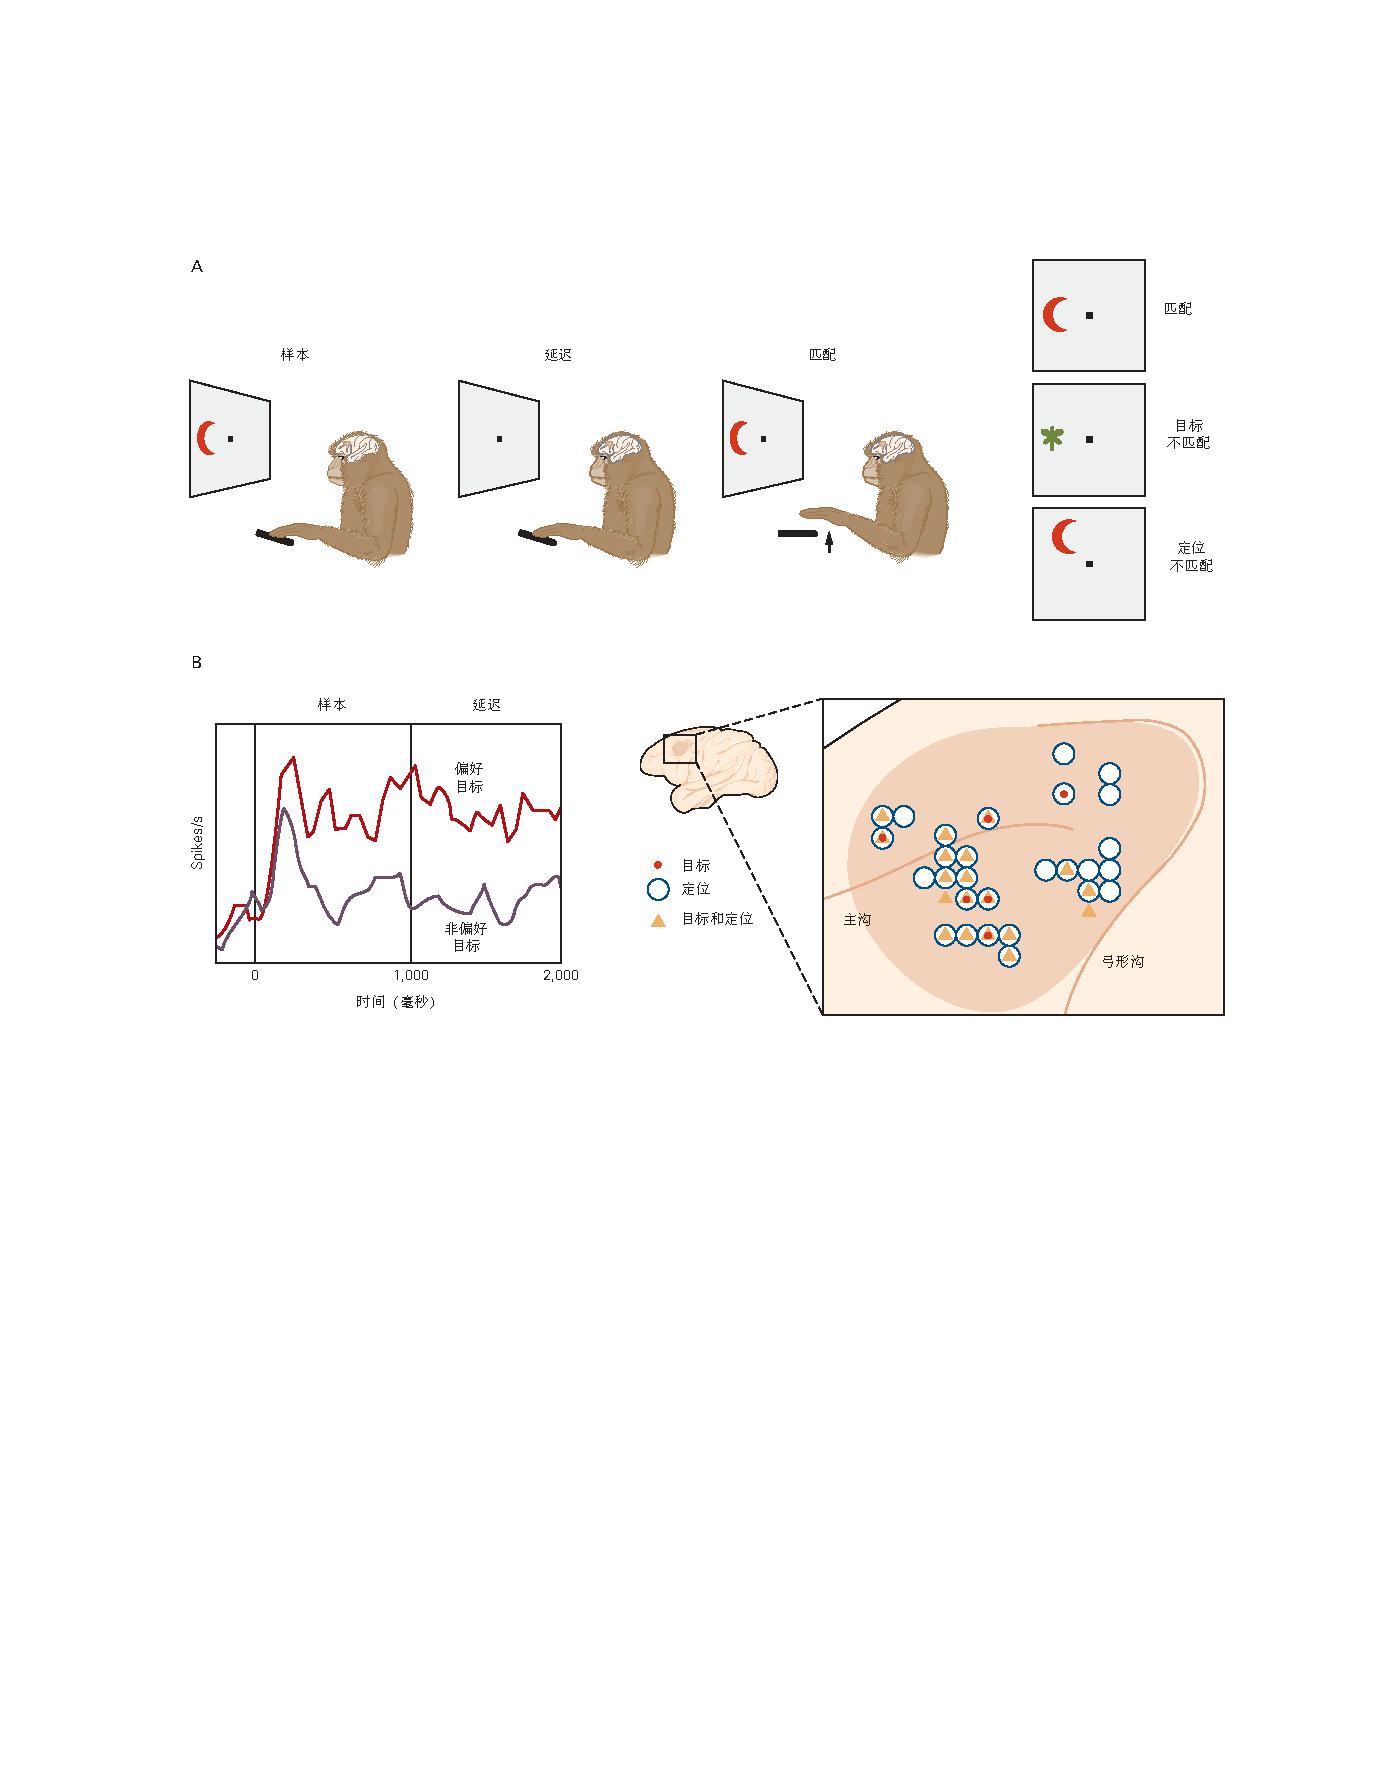
\includegraphics[width=1.0\linewidth]{chap52/fig_52_1}
	\caption{前额叶皮层维持工作记忆。(经 Rainer、Asaad 和 Miller 1998 许可改编。)\cite{rainer1998memory}。
		\textbf{A.} \textit{前额叶皮层}在维持工作记忆信息中的作用通常在猴子中使用电生理学方法结合\textit{延迟样本匹配}对任务进行评估。
		在这种类型的任务中,当猴子抓住反应杆并在视觉上固定计算机屏幕中央的一个小目标时,每个试验就开始了。
		初始视觉刺激(样本)会被简要呈现,并且必须保留在工作记忆中,直到下一个刺激(匹配)出现。
		在这里所示的任务中,猴子需要记住样本(“什么”)及其位置(“哪里”),并且只有在响应两个维度上匹配的刺激时才释放杠杆。
		\textbf{B.} 在延迟期间,猴子外侧前额叶皮层的神经放电率通常保持在基线以上,并代表对刺激类型(什么)、位置(何处)以及两者的整合(什么和何处)的相应。
		如图所示,左侧是前额叶神经元响应首选物体(神经元对此反应强烈)和非首选物体(神经元对其反应最小)的活动。
		当猴子看着喜欢的物体(样本)和延迟期间,活动都很活跃。
		在右图中,符号代表神经元保存每种类型信息(内容、地点、内容和地点)的记录位点。
		通常,在一个部位会发现多种类型的神经元。
		因此,许多符号重叠,有些符号表示多个神经元。}
	\label{fig:52_1}
\end{figure}


因此,工作记忆涉及激活存储在根据信息内容而变化的专门皮层区域中的信息表征,以及激活前额叶皮层中的一般控制机制。
工作记忆中的前额叶控制信号进一步依赖于与纹状体的相互作用和来自中脑的上行多巴胺能输入。



\subsection{存储在短期记忆中的信息有选择地转移到长期记忆中}

在 20 世纪 50 年代中期,对因治疗癫痫而接受双侧海马体和内侧颞叶邻近区域切除术的患者进行的研究中,出现了关于长期记忆神经基础的令人震惊的新证据。
第一个也是研究最多的病例是一位名叫\textit{亨利$\cdot$莫莱森}的患者由心理学家布布伦达·米尔纳和外科医生威廉·斯科维尔研究。


\textit{亨利$\cdot$莫莱森}多年来,他一直患有无法治愈的颞叶癫痫,其原因是 7 岁时因自行车事故造成脑损伤。
成年后,他的癫痫发作使他无法工作或过正常的生活,在 27 岁时,他接受了手术。
\textit{斯科维尔}切除了被认为与癫痫发作有关的大脑区域,包括海马结构、杏仁核和双侧颞叶皮层的多模式关联区域的部分(图~\ref{fig:52_2})。
手术后,\textit{亨利$\cdot$莫莱森}的癫痫发作得到了更好的控制,但他留下了毁灭性的记忆缺陷(或健忘症)。
\textit{亨利$\cdot$莫莱森}的缺陷之所以如此引人注目,是因为它的特殊性。


\begin{figure}[htbp]
	\centering
	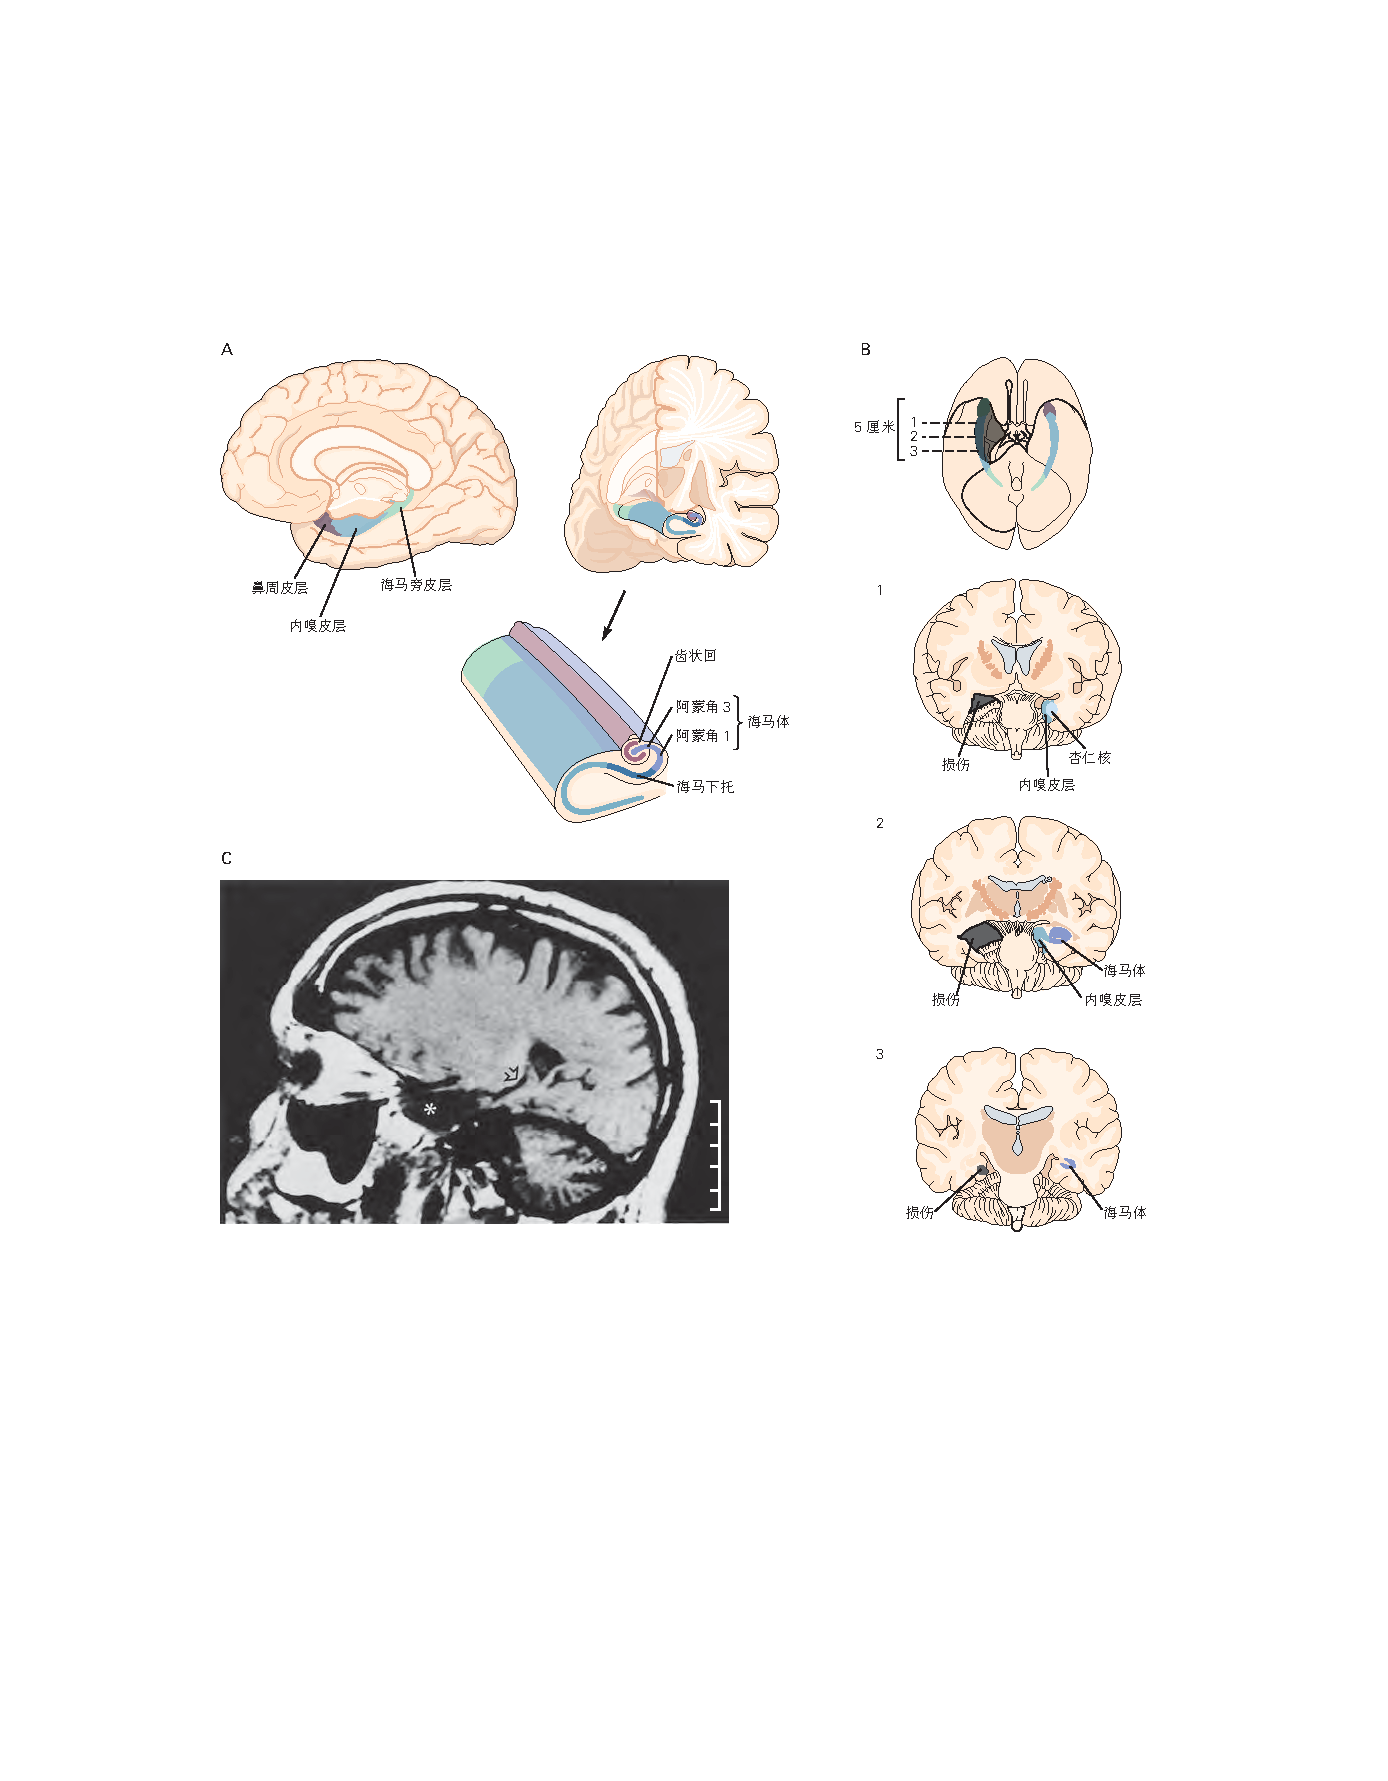
\includegraphics[width=1.0\linewidth]{chap52/fig_52_2}
	\caption{内侧颞叶和记忆存储。
		\textbf{A.} 内侧颞叶的关键组成部分对于记忆存储很重要。
		\textbf{B.} 从大脑腹侧表面观察(左半球位于图像右侧),被称为\textit{亨利$\cdot$莫莱森}的患者的颞叶区域被切除(灰色阴影),从大脑的腹侧表面观察(左半球在图像的右侧)。
		手术是双侧、单阶段的手术,但为了说明从左半球(图像右侧)移除的结构,此处显示了完整的左半球。
		病变的纵向范围显示在大脑的腹侧视图中(上)。
		横截面 1 到 3 显示了从叫\textit{亨利$\cdot$莫莱森}身上切除的大脑区域的估计范围\cite{corkin1997hm}。
		\textbf{C.} \textit{亨利$\cdot$莫莱森}大脑左侧矢状切面的\textit{磁共振图像(MRI)}扫描。
		面板右侧的校准条具有 1 厘米增量。
		扫描中央区域的星号表示前颞叶的切除部分。
		附近的箭头指向海马结构脑室内部分的剩余部分。
		双侧可见约 2 厘米的保留海马结构。
		还要注意小脑扩大的叶空间的严重退化。\cite{corkin1997hm}。}
	\label{fig:52_2}
\end{figure}


他仍然具有正常的工作记忆,持续几秒或几分钟,这表明内侧颞叶对于瞬时记忆来说不是必需的。
他对手术前发生的事件也有长期记忆。
例如,他记得自己的名字、从事的工作和童年经历。
此外,他保留了对语言的掌握,包括词汇,这表明语义记忆(关于人、地方和事物的事实知识)得以保留。
他的智商没有变化,在正常范围内。


\textit{亨利$\cdot$莫莱森}现在所缺乏,而且严重缺乏的是将新信息转移到长期记忆中的能力,这种缺陷被称为\textit{顺行性遗忘症}。
他无法长时间保留有关他刚刚遇到的人、地点或物体的信息。
当被要求记住一个新的电话号码时,由于\textit{亨利$\cdot$莫莱森}有完整的工作记忆,他可以立即重复几秒钟到几分钟。
但是当分心时,即使是短暂的,他也会忘记号码。
\textit{亨利$\cdot$莫莱森}无法认出他在手术后遇到的人,即使他一次又一次地遇到他们。
几年来,他每个月都见到米尔娜,但每次她走进房间,他的反应就好像他以前从未见过她一样。
\textit{亨利$\cdot$莫莱森}的这种情况不唯一,
所有内侧颞叶边缘联合区双侧广泛病变的患者都表现出类似的长期记忆缺陷。


\textit{亨利$\cdot$莫莱森}这是一个历史性的案例,因为他的缺陷首次提供了记忆与内侧颞叶(包括海马体)之间的第一个明确联系。
\textit{拉里$\cdot$斯奎尔}和其他人对海马体脑损伤患者的后续研究证实了海马体在记忆中的核心作用。
观察结果表明,\textit{亨利$\cdot$莫莱森}和其他患有内侧颞叶损伤的人在新记忆的形成方面存在严重缺陷,而旧记忆的提取基本保持完整,这表明记忆必须随着时间的推移从海马体和内侧颞叶转移到其他大脑结构。
这些研究提出了四个核心问题,这些问题至今仍在推动记忆研究:首先,内侧颞叶记忆系统的功能作用是什么?
第二,不同次区域在这个体系中的作用是什么?
第三,这些子区域如何与其他大脑回路一起工作以支持不同形式的记忆?
第四,海马依赖性记忆最终存储在哪里?



\section{内侧颞叶对情景式长期记忆至关重要}

关于\textit{亨利$\cdot$莫莱森}的一个重要发现是:长期记忆的形成只对某些类型的信息受损。
% 情景式长期记忆,而对技能不影响
\textit{亨利$\cdot$莫莱森}和其他内侧颞叶受损的患者能够像健康受试者一样形成和保留某些类型的持久记忆。


例如,\textit{亨利$\cdot$莫莱森}在镜子里看着星星和他的手,学会了画出星星的轮廓(图~\ref{fig:52_3})。
就像健康的受试者学习重新映射手眼协调一样,\textit{亨利$\cdot$莫莱森}最初犯了很多错误,但经过几天的训练,他的表现没有错误,可以与健康受试者相媲美。
然而,他并没有自觉地记得自己曾经完成过这项任务。


\begin{figure}[htbp]
	\centering
	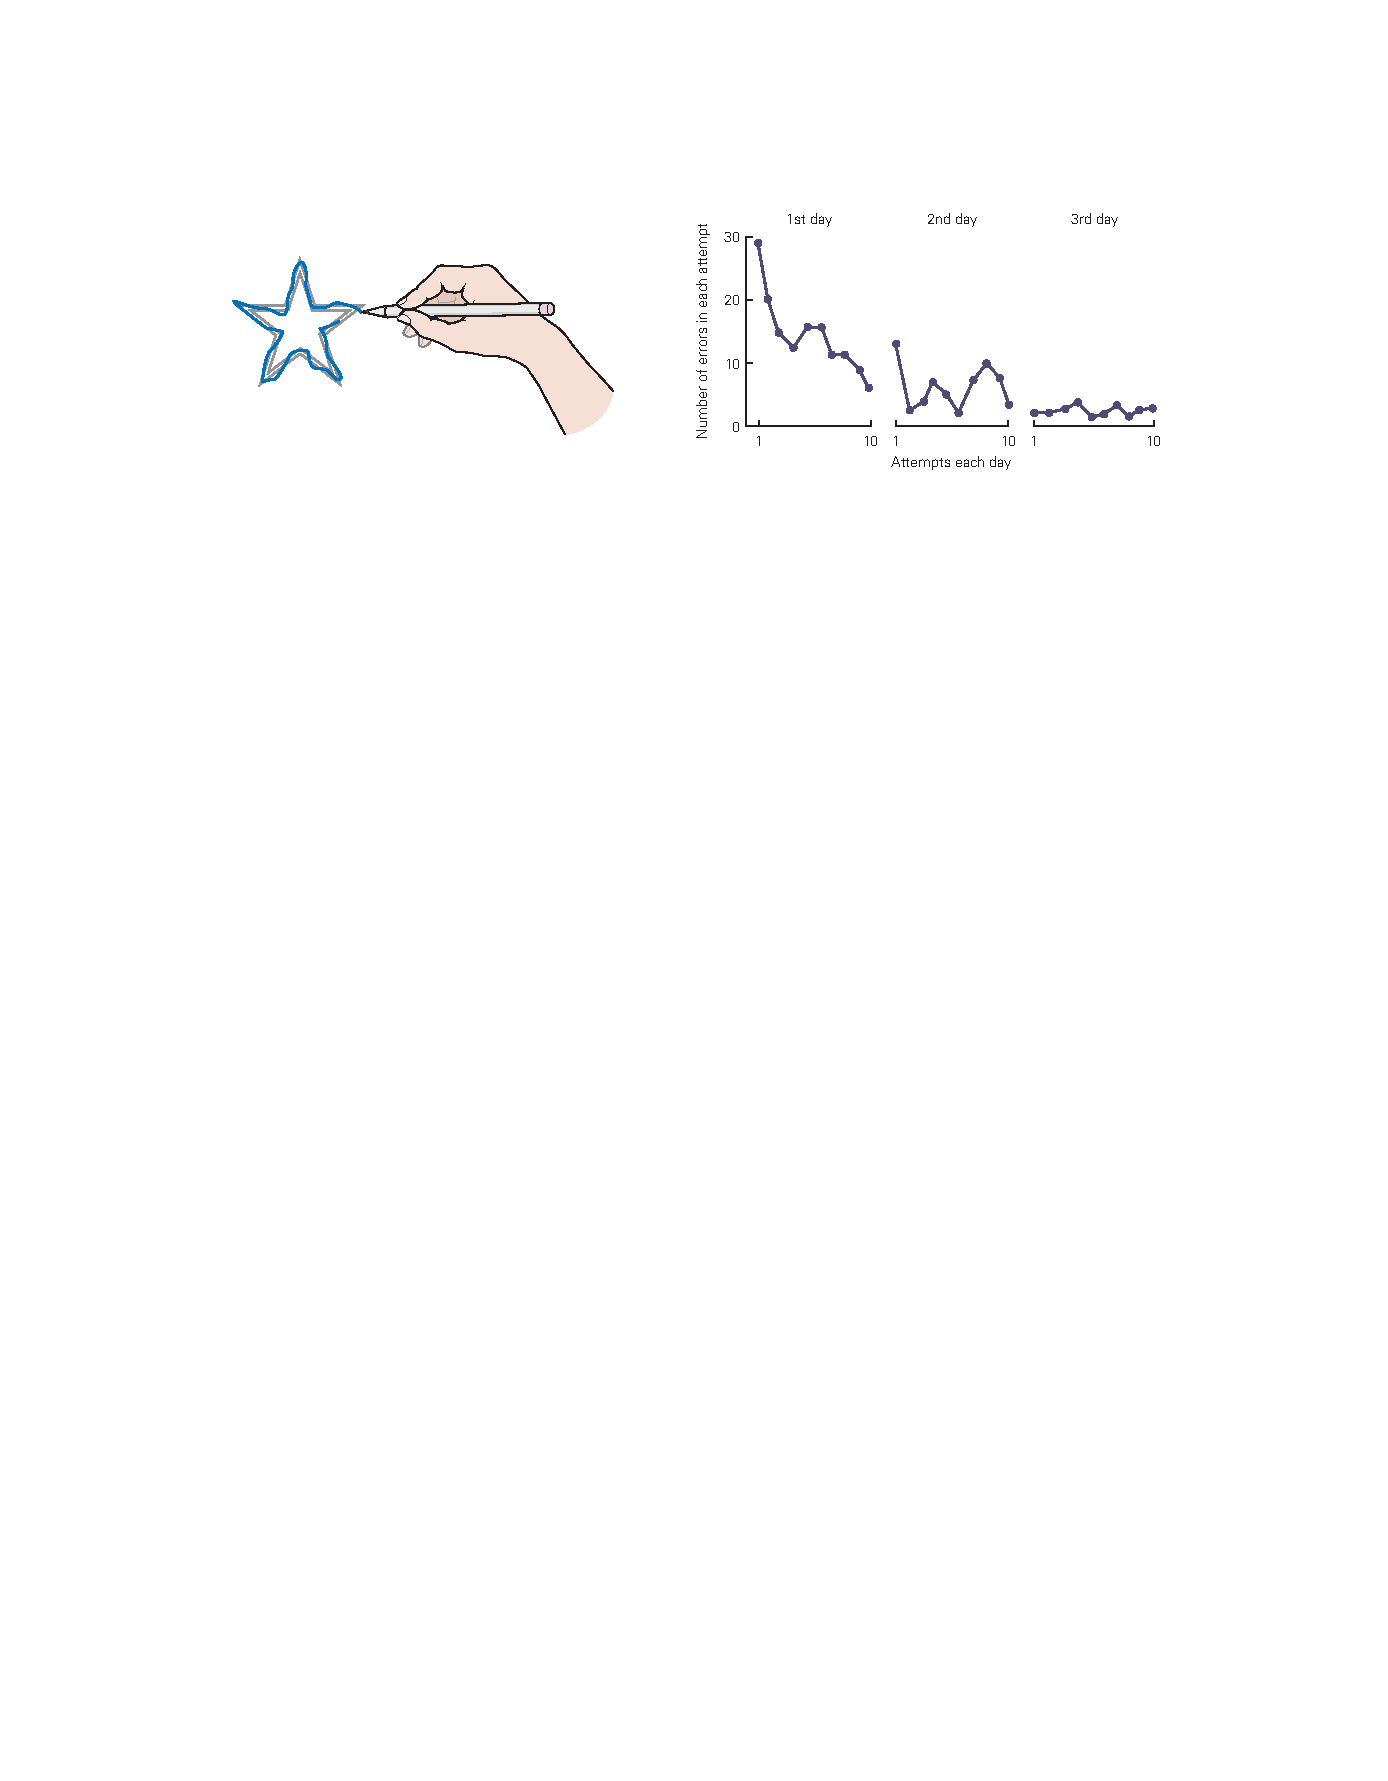
\includegraphics[width=1.0\linewidth]{chap52/fig_52_3}
	\caption{健忘症患者叫\textit{亨利$\cdot$莫莱森}可以学习熟练的动作。
		他被教导一边在镜子里观察自己的手,在一颗星星的两个轮廓之间描画。
		该图绘制了每次尝试期间他在绘制星星时偏离轮廓的次数。
		与健康受试者一样,尽管\textit{亨利$\cdot$莫莱森}不记得执行过该任务,但通过反复尝试,他的表现有了很大改善\cite{blakemore1977mechanics}。}
	\label{fig:52_3}
\end{figure}


健忘症患者的长期记忆形成不仅限于运动技能。
这些患者保留了简单的反射性学习,包括习惯化、敏感化和某些形式的条件反射(将在本章后面讨论)。
此外,他们能够提高他们在某些感知和概念任务上的表现。
例如,他们擅长一种称为启动的记忆形式,在这种记忆中,通过先前的接触可以改善对单词或目标的感知或对单词或目标含义的访问。
因此,当仅显示先前学习过的单词的前几个字母时,健忘症患者能够产生与正常受试者相同数量的学习过的单词,即使健忘症患者对最近遇到的单词没有有意识的记忆(图~\ref{fig:52_4})。


\begin{figure}[htbp]
	\centering
	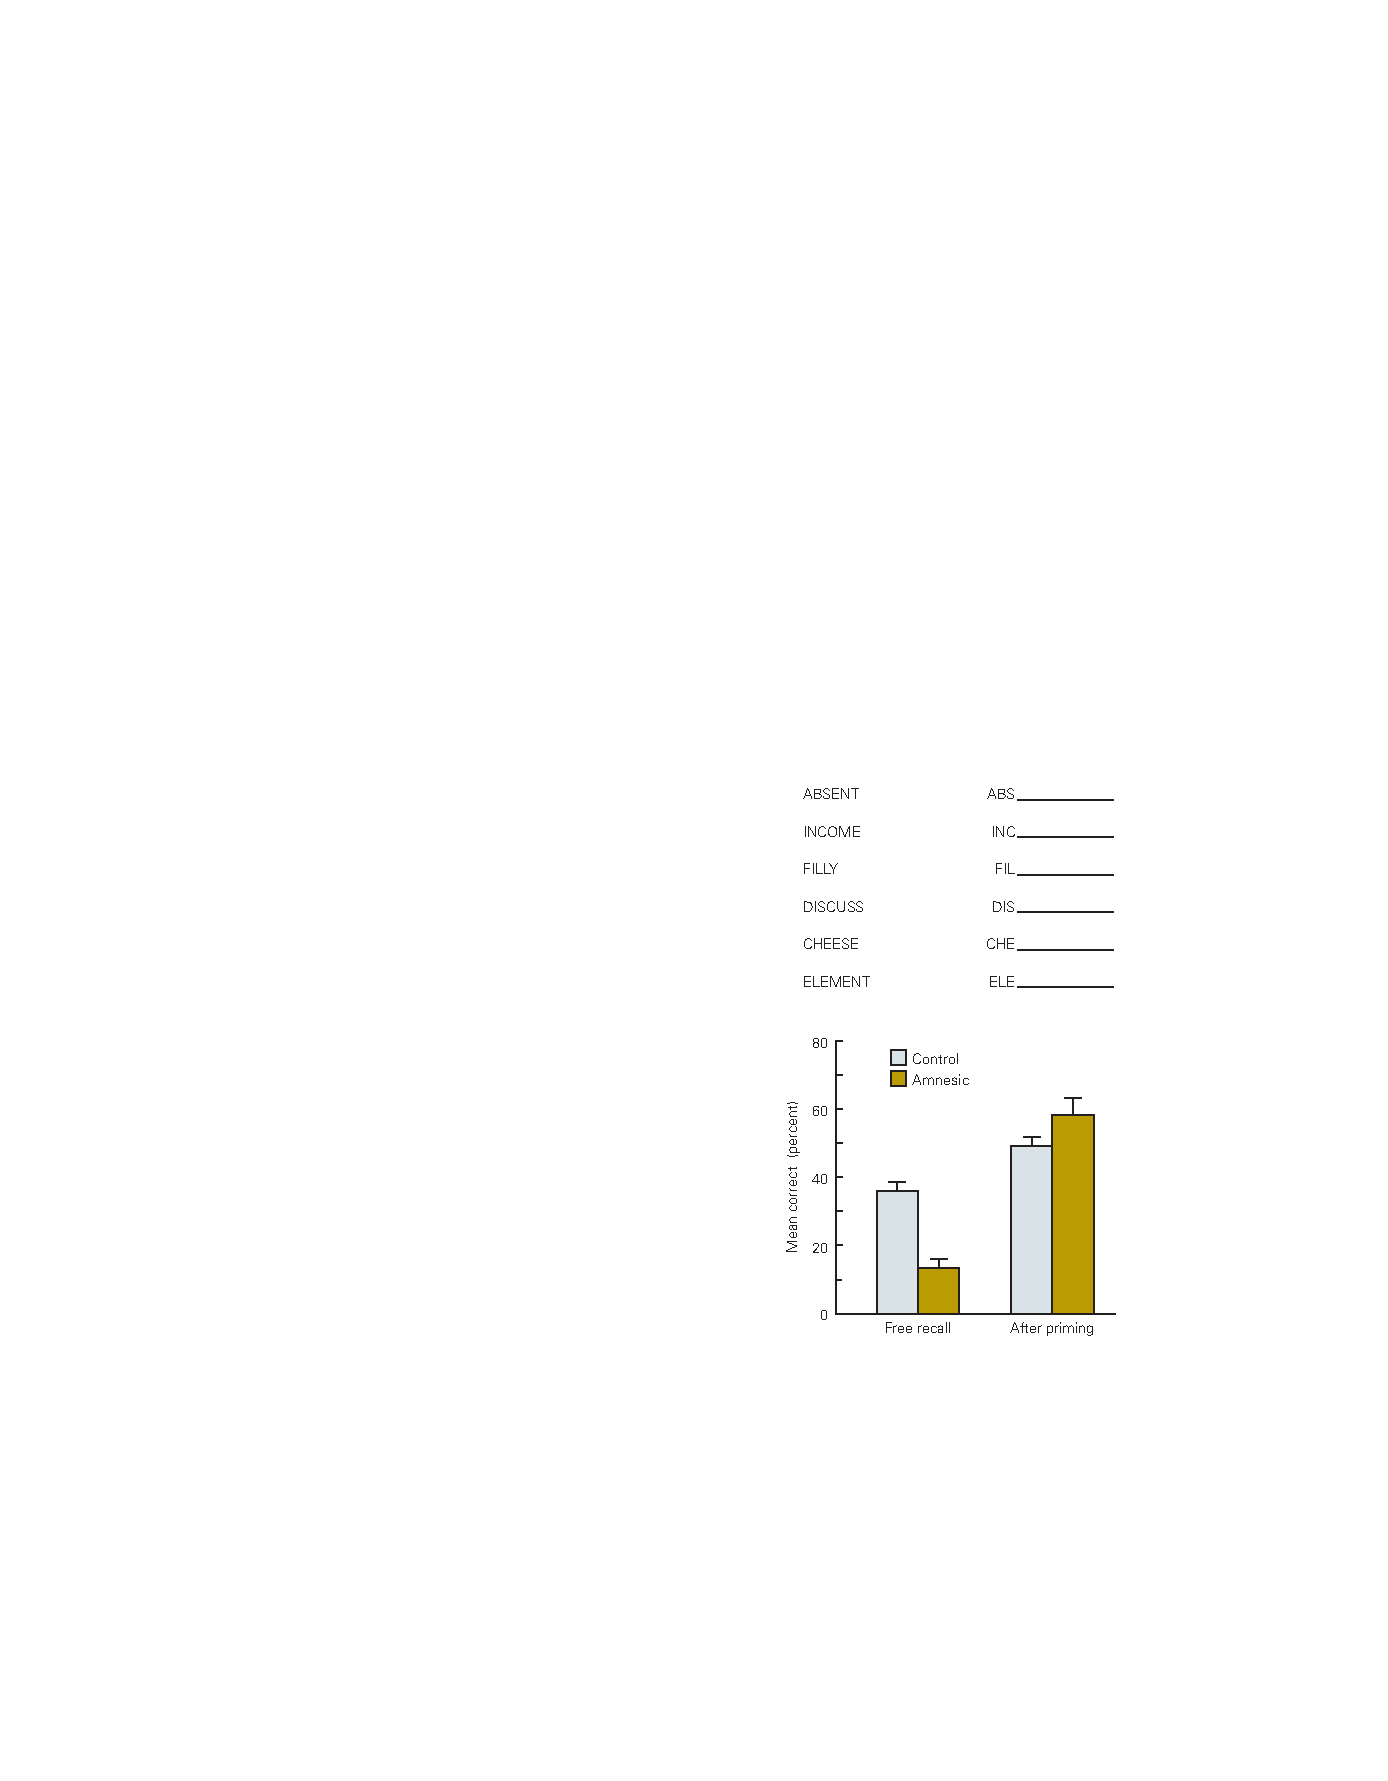
\includegraphics[width=0.47\linewidth]{chap52/fig_52_4}
	\caption{健忘症受试者在两种情况下回忆单词的能力不同。
		受试者被出示常用单词,然后被要求回忆这些单词。
		健忘症患者在\textit{自由回忆}期间在这项测试中表现不佳。
		然而,当健忘症受试者被赋予单词的前三个字母,并被指示形成脑海中的第一个单词(单词完成)时,健忘症受试者的表现与正常受试者一样好。
		先前未出现的单词在单词完成条件下的基线猜测率为9\%\cite{squire1987memory}。}
	\label{fig:52_4}
\end{figure}


健忘症患者选择性表现受损的模式引发了如何对这些不同形式的记忆进行分类的问题:
区分内侧颞叶损伤后存活的记忆和未损伤记忆的关键特征是什么?
\textit{斯奎尔}及其同事的早期理论表明,一个关键因素可能是有意识的认知:对内侧颞叶的损伤似乎会损害可以被有意识地访问并可以用言语报告或表达的记忆形式,而保留了不能被访问的记忆形式。
因此,依赖于内侧颞叶的记忆通常被称为外显(或陈述性)记忆。
外显记忆可进一步分为情景记忆(个人经历的记忆或自传体记忆)和语义记忆(对事实的记忆)。
情景记忆是指我们能够及时记住瞬间的丰富细节,包括有关发生的事情、时间和地点的信息。
例如,情景记忆用于回忆我们昨天看到了春天的第一朵花,或者几个月前我们听到了贝多芬的《月光奏鸣曲》。
语义记忆用于回忆单词或概念的含义,以及其他事实。


认知心理学家通过使用记忆表达方式不同的任务,在健康受试者的不同记忆形式之间发现了类似的区别。
一种类型是一种无意识的记忆形式,在执行任务时很明显。
这种形式的记忆通常称为内隐记忆(也称为非陈述性或程序性记忆)。
内隐记忆通常以自动方式表现出来,受试者很少有意识地进行处理。
不同的形式会引起启动、技能学习、习惯记忆和条件反射(图~\ref{fig:52_5})。
外显记忆被认为是高度灵活的;
在不同的情况下,可以关联多条信息。
然而,内隐记忆与学习发生的原始条件紧密相关。


\begin{figure}[htbp]
	\centering
	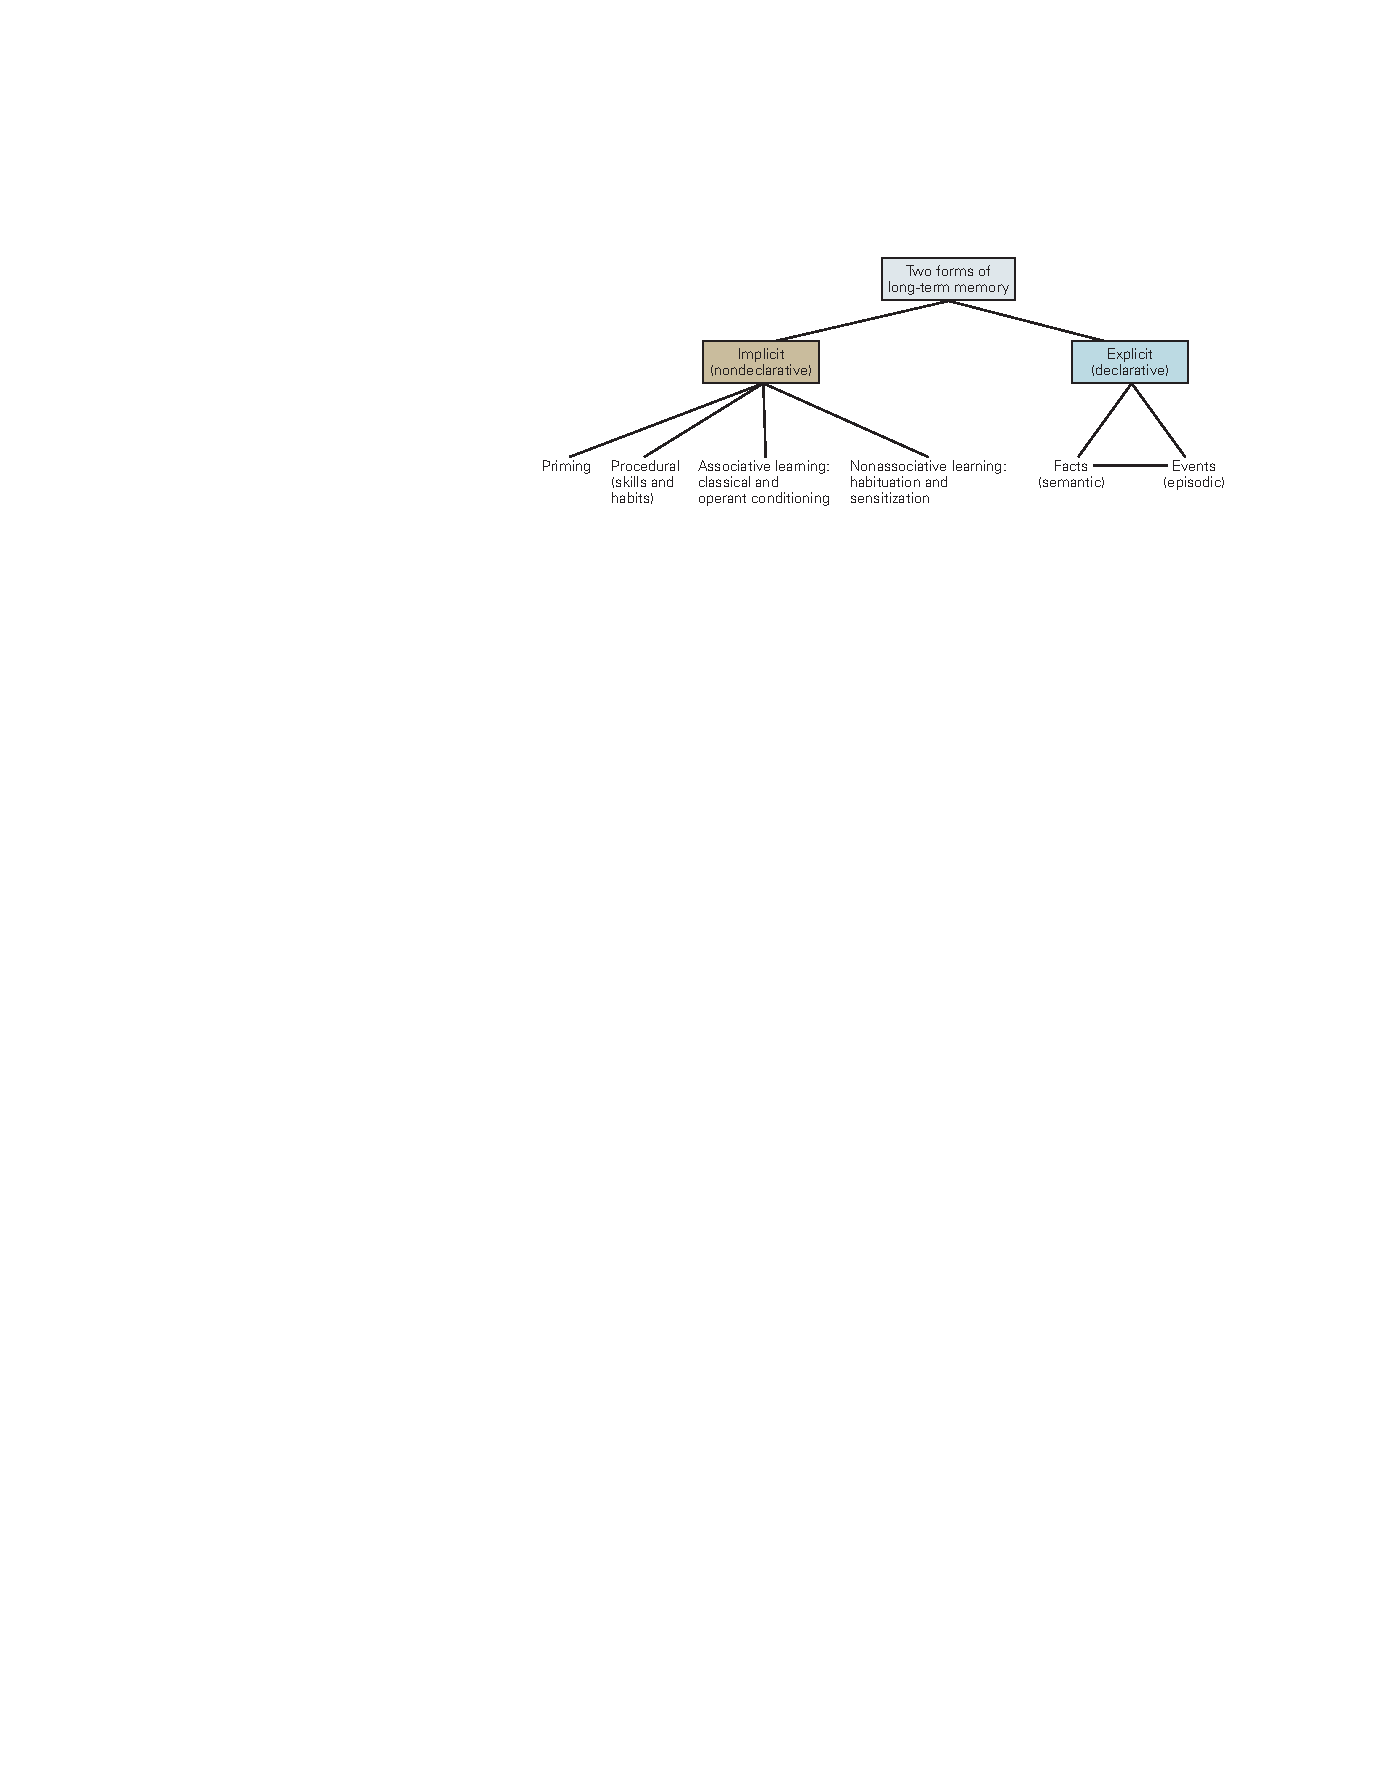
\includegraphics[width=0.91\linewidth]{chap52/fig_52_5}
	\caption{长期记忆通常分为外显记忆(记忆是口头报告的)或内隐记忆(记忆是通过无意识的行为表达的)。}
	\label{fig:52_5}
\end{figure}


术语“外显记忆”和“内隐记忆”用于描述两种广泛的记忆形式,这两种记忆的标志性行为特征和神经基础不同。
这些形式的记忆可以并行获得。
例如,一个人可能会对昨天进入一家面包店时闻起来有多香形成明确的记忆,而与此同时,一个人可能会在看到面包店的照片后产生一种自动条件反射,即流口水增加。
此外,我们现在认为,这些形式的记忆虽然截然不同,但通常会相互作用以支持行为,尽管它们相互作用的确切性质和范围是正在进行的调查的主题。


关于意识意识在记忆中的作用以及它是否确实是内侧颞叶支持的记忆的必要特征,存在持续的争论。
这些争论是由越来越多的研究推动的,这些研究表明外显记忆所需的相同内侧时间回路对于某些形式的内隐记忆也是必需的(如下所述)。
事实上,虽然情景记忆通常通过要求受试者报告他们记忆的内容来评估,但目前尚不清楚有意识的可访问性是否是记忆本身的一个组成部分。
尽管如此,内隐记忆和外显记忆之间的区别在区分记忆形式方面发挥了重要的历史作用,并且仍然为考虑记忆的神经基础提供了一个富有成效的框架。
因此,我们在这里使用术语“外显记忆”和“内隐记忆”来区分这两种记忆形式以及它们所基于的主观体验和行为的类别。
在接下来的部分中,我们将重点关注情景记忆,它一直是健忘症患者和健康个体的大量认知神经科学研究的目标。



\subsection{情景记忆处理涉及编码、存储、检索和整合}

情景记忆已得到广泛研究,为理解大脑如何构建、存储和检索生活中的情景细节提供了一个窗口。
我们现在知道大脑没有单一的长期情景记忆存储。
相反,任何知识项的存储都广泛分布在许多大脑区域中,这些区域处理记忆内容的不同方面,并且可以独立访问(通过视觉、口头或其他感官线索)。
其次,情景记忆至少由四种相关但截然不同的处理类型介导:编码、存储、巩固和检索。


编码是在新记忆形成过程中最初获取和处理新信息的过程。
这种处理的程度对于确定所学材料的记忆程度至关重要。
为了让记忆持久并被牢记,传入的信息必须经过心理学家\textit{弗格斯$\cdot$克雷克}和\textit{罗伯特$\cdot$洛哈特}所称的“深度”编码。
这是通过注意信息并将其与已经建立的记忆相关联来实现的。
当一个人有动力去记忆时,记忆编码也会更强,无论是因为信息具有特定的情感或行为相关性(例如,在愉快的第一次约会时记得特别美味的一餐)还是因为信息本身是中性的,但与某种有意义的事物相关联(例如,记住那家餐馆的位置)。


存储是指新获取的信息随着时间的推移被保留为持久记忆的神经机制和位点。
长期存储的显着特征之一是它似乎具有几乎无限的容量。
相比之下,工作记忆的存储空间非常有限;
心理学家认为,人类的工作记忆在任何时候只能容纳少量的信息。


整合是将临时存储且仍不稳定的信息转换为更稳定形式的过程。
正如我们将在接下来的两章中了解到的,巩固涉及基因表达和蛋白质合成,从而引起突触的结构变化。


最后,检索是回忆存储信息的过程。
它涉及回想起存储在不同站点中的不同类型的信息。
记忆的检索很像感知。
它是一个建设性的过程,因此容易受到扭曲,就像感知受到幻觉的影响一样(框~\ref{box:52_1})。
当记忆被检索时,它会再次激活,为旧记忆提供再次编码的机会。
由于检索是建设性的,因此检索到的记忆的重新编码可能与原始记忆不同。
例如,重新编码可以包括来自旧存储器的信息以及检索该信息的新上下文。
这种重新编码允许将不同时刻的记忆在内存中连接起来,但它也为内存中的错误打开了大门,正如本章后面所讨论的。


当检索提示提醒个体连接编码体验元素的事件的情景性质时,信息检索是最有效的。
例如,在一个经典的行为实验中,\textit{克雷格$\cdot$巴克莱}及其同事要求一些受试者对诸如“那个人举起钢琴”之类的句子进行编码。
在后来的检索测试中,“重的东西”比“声音好听的东西”更能有效地回忆钢琴。
然而,其他受试者编码了“那个人调好了钢琴”这句话。
对他们来说,“声音好听的东西”是比“重的东西”更有效的钢琴检索提示,因为它更好地反映了最初的体验。
检索,尤其是外显记忆的检索,也部分依赖于工作记忆。



\subsection{情景记忆涉及内侧颞叶和联合皮层之间的相互作用}

尽管过去几十年对健忘症患者的研究加深了我们对各种类型记忆的理解,但内侧颞叶损伤会影响记忆的所有四种操作(编码、存储、巩固和检索),因此通常很难辨别内侧颞叶如何对每个都有贡献。
\textit{功能性磁共振成像}允许我们在建立新记忆或检索现有记忆的过程中扫描大脑活动,从而识别在不同过程中活跃的特定区域(第~\ref{chap:chap6}~章)。


使用功能性核磁共振成像研究编码的常用方法是后续记忆范式。
在一个典型的后续记忆任务中,人类受试者在使用功能性核磁共振成像扫描时一次观察一系列刺激(例如,单词或图片),通常是在从事掩饰任务(例如,确定图片是否为彩色或黑白)。
然后在扫描仪之外测试受试者对刺激的记忆,使研究人员能够将所有编码事件分类为后来记住的事件和后来忘记的事件。
\textit{功能性磁共振成像}扫描显示,在编码过程中,与被遗忘的项目相比,被记住的项目与海马区的活动更强相关。
这种差异在大脑的其他部分,包括前额叶、逆行区和顶叶皮层的同时活动中也很明显。
通常,在记忆编码过程中,这些区域的活动与海马体的活动时时刻刻都在发生变化,这表明这些区域在功能上是相互联系的(图~\ref{fig:52_6})。


\begin{figure}[htbp]
	\centering
	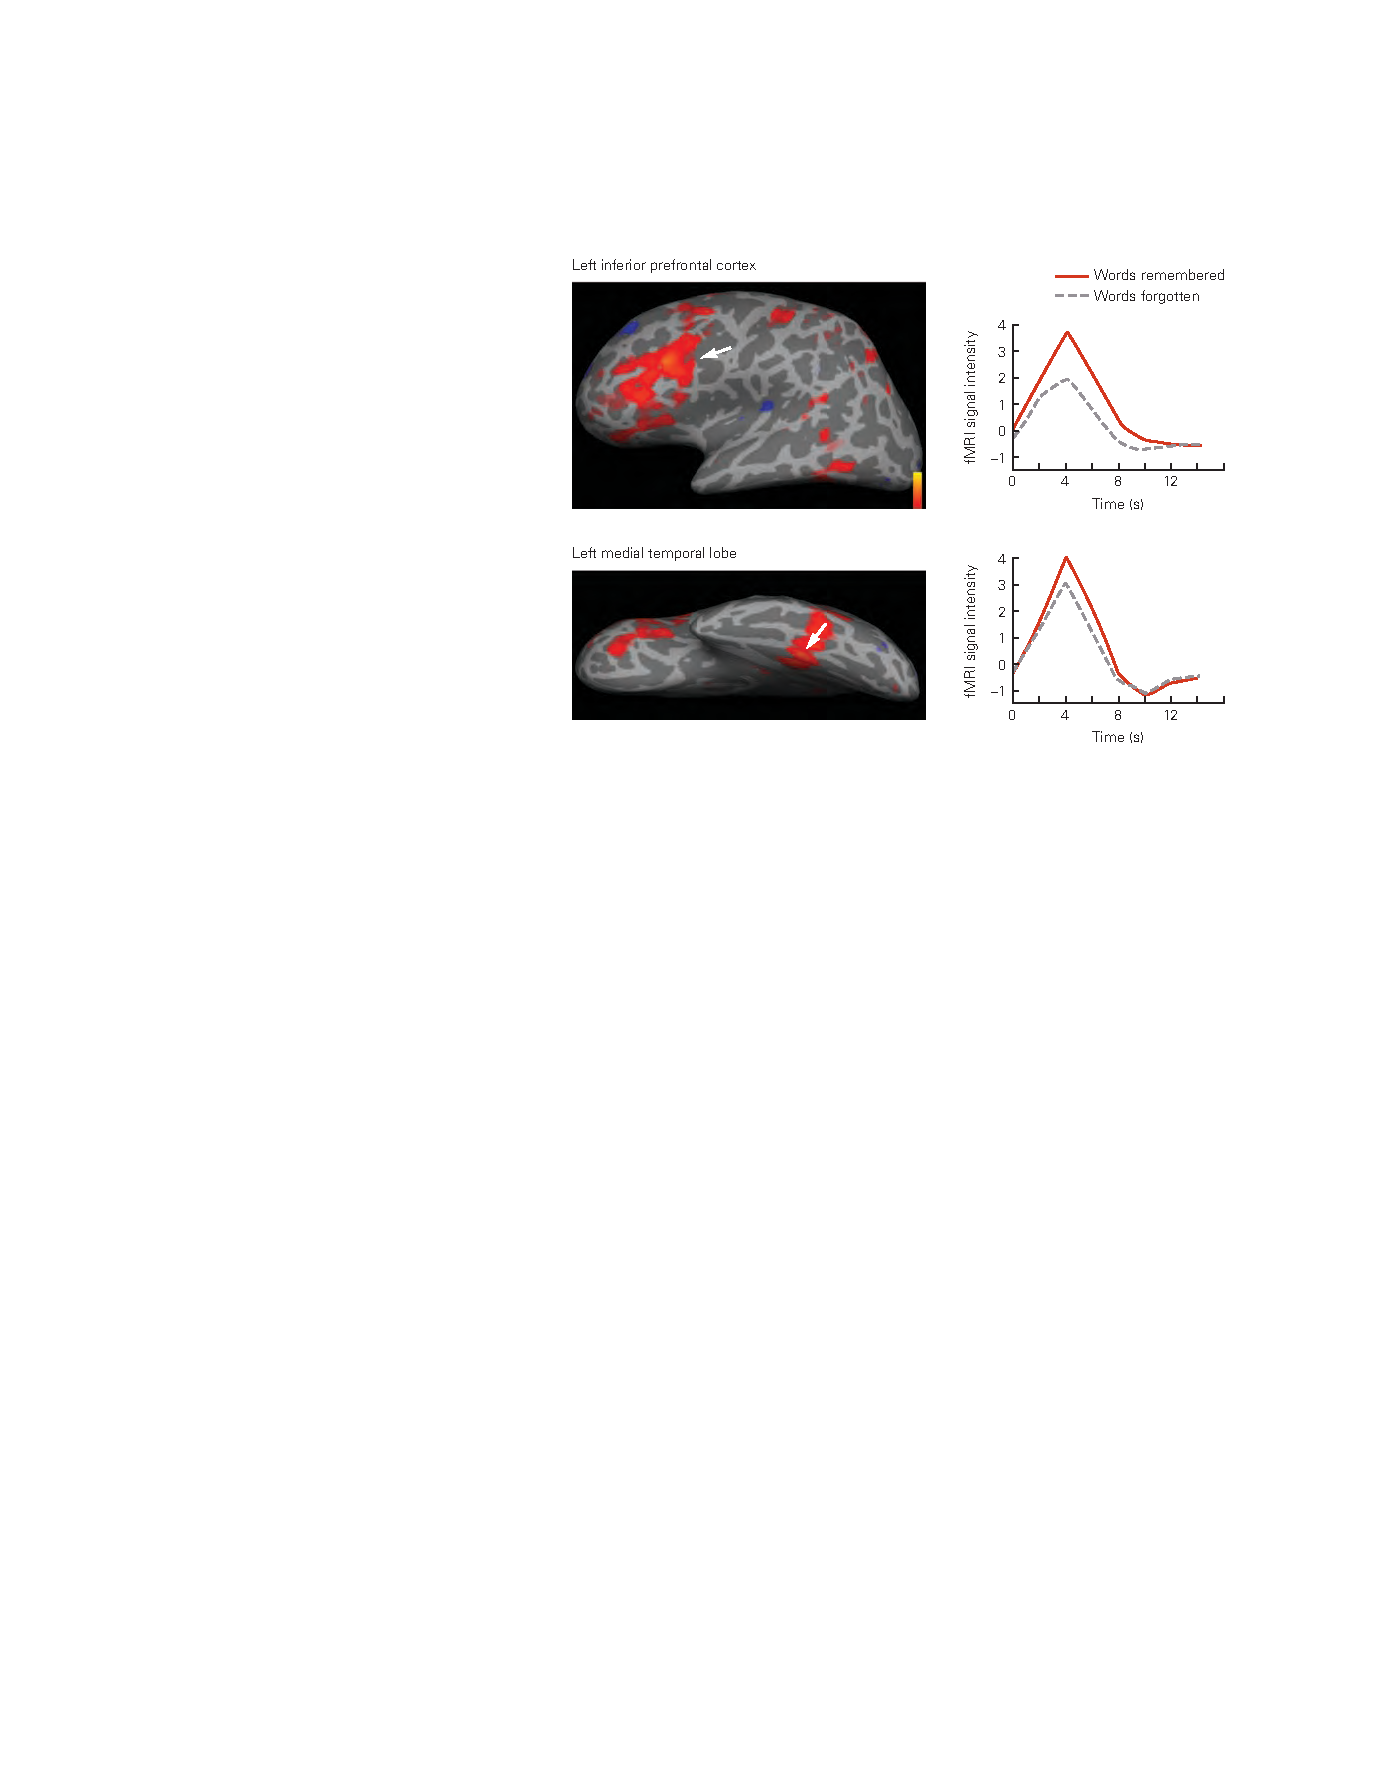
\includegraphics[width=0.81\linewidth]{chap52/fig_52_6}
	\caption{在这里说明的研究中,使用\textit{功能性核磁共振成像}测量了视觉事件(单词呈现)编码过程中的神经活动。
		随后,测试了对所学单词的回忆,并将每个单词归类为记住或遗忘。
		然后将编码期间进行的扫描分为两组:一组是在编码后来被记住的单词时进行的,另一组是在编码后来被遗忘的单词时进行的。
		在编码后来记住的单词时,左前额叶皮层和内侧颞叶区域的活动比后来忘记的单词(位置用白色箭头表示)更活跃。
		右边是在这些区域中观察到的\textit{功能性磁共振成像}反应,用于后来记住的单词和后来忘记的单词\cite{wagner1998building}。}
	\label{fig:52_6}
\end{figure}


这些功能性核磁共振成像研究结果,连同健忘症患者的研究结果,为海马体在编码情景记忆中的重要作用提供了强有力的支持。
\textit{功能性核磁共振成像}的发现还扩展了健忘症患者的发现,表明情景记忆的成功形成取决于额顶叶网络和内侧颞叶之间的相互作用。
然而,由于内侧颞叶是一个大型结构,关键目标是了解其不同分区的作用。
此类信息由使用更强大的大脑扫描技术的更高分辨率的\textit{功能性磁共振成像}研究提供。
这些研究表明,海马体内外的不同亚区对记忆编码的不同方面有贡献。
因此,虽然海马体周围的一些皮质区域对于物体识别(鼻周皮层)特别重要,但其他区域对于编码空间上下文(海马旁皮层)非常重要。
这些皮层区域为海马体提供了强大的(但间接的)输入,海马体被认为将空间和物体信息结合在一起,形成统一的记忆。


内侧颞叶和广泛分离的皮层区域之间的相互作用也是记忆巩固和检索的核心。
最初认为海马体对于检索并不重要,因为内侧颞叶被手术切除的患者叫\textit{亨利$\cdot$莫莱森}仍然可以回忆起童年记忆。
事实上,早期的观察表明直到\textit{亨利$\cdot$莫莱森}手术前几年,他都能回忆起他生活中的许多经历。
对\textit{亨利$\cdot$莫莱森}和其他内侧颞叶受损的遗忘症患者的这些观察表明,旧的记忆必须通过与内侧颞叶的相互作用最终存储在其他各种皮层区域中。
然而,尽管像叫\textit{亨利$\cdot$莫莱森}这样的海马损伤患者有一定的回忆旧记忆能力,有证据表明这些患者的记忆回忆程度可能受损。
目前的想法表明,存在一个涉及多个大脑区域的用于合并和检索的分布式回路,海马体在编码和检索过程中的关联绑定中起着至关重要的作用。
皮层区域作为构成记忆的独立信息元素的长期储存库,以及记忆本身内容的受控检索和重新激活。


与编码研究一样,情景知识检索研究涉及联合皮层、额顶叶网络和内侧颞叶的特定区域。
与情景记忆相关的上下文或事件细节的检索也涉及海马体的活动,内侧颞叶检索过程促进了编码过程中存在的新皮层表征的激活。


由于与大脑活动相关的血流变化的时间过程相对较慢,\textit{功能性磁共振成像}扫描的时间分辨率相当有限。
为了获得更高的大脑活动时间分辨率,研究人员可以使用细胞外电极记录人脑的电活动。
这种记录很少见,只有在已经因医学原因(例如严重癫痫)接受脑部手术的人类患者中才有可能,当时使用电极植入来定位癫痫发作的部位。
在一项研究中,使用放置在内侧颞叶和皮层其他区域的硬膜下电极测量\textit{颅内脑电图}信号。
受试者首先学习成对单词之间的关联,然后必须检索这些关联的记忆。
记忆的恢复与海马体中的神经活动有关,并与颞叶联合皮层中的神经活动相关,颞叶联合皮层是一个涉及语言和多感官整合的区域。
这种耦合的神经活动与皮层模式的重新激活有关,这些模式最初是在参与者第一次记住单词对时观察到的。
这一发现提供了记忆初始编码期间在海马体中观察到的神经活动与检索期间时间关联皮层中后来耦合活动之间的联系。
许多人体功能成像研究报告了在检索过程中重新激活编码模式的相关观察,记录了这种影响的普遍性。
与情景记忆的编码一样,提取涉及内侧颞叶和分布式皮层区域之间的复杂相互作用,包括额顶叶网络和其他高层关联区域。



\subsection{情景记忆有助于想象力和目标导向的行为}

记忆使我们能够利用过去的经验来预测未来的事件,从而促进适应性行为。
就像记忆的检索一样,对未来事件的想象涉及从记忆中构建细节。
记忆和想象之间可能存在联系的第一份报告来自患者 K.C. 的个案研究,正如\textit{安道尔$\cdot$图威}在 1985 年报道的那样。
由于海马体和内侧颞叶受损,他表现出典型的毁灭性失忆症。
与患者叫\textit{亨利$\cdot$莫莱森}相似,他完全缺乏情景记忆,但语言和非情景功能未受损。
图尔文的研究进一步表明,这种脑损伤与丧失想象未来事件的能力有关。
当被问到他第二天会做什么时,K.C. 无法提供详细信息。


海马体在想象未来事件中的重要性也体现在\textit{功能性磁共振成像}研究中。
此类研究检查了健康人的大脑活动,将受试者被要求记住过去的事件(例如,想想你去年的生日)时的活动与他们想象未来事件(例如,想象明年夏天的海滩度假)时的活动进行比较 )。
受试者被要求报告想到的事件的任何生动细节。
\textit{功能性核磁共振成像}扫描显示在记忆检索和对未来事件的想象过程中活跃的大脑区域网络中存在惊人的重叠。
该网络包括海马体、前额叶皮层、后扣带皮层、压后皮层以及外侧顶叶和颞叶区域(图~\ref{fig:52_7})。


\begin{figure}[htbp]
	\centering
	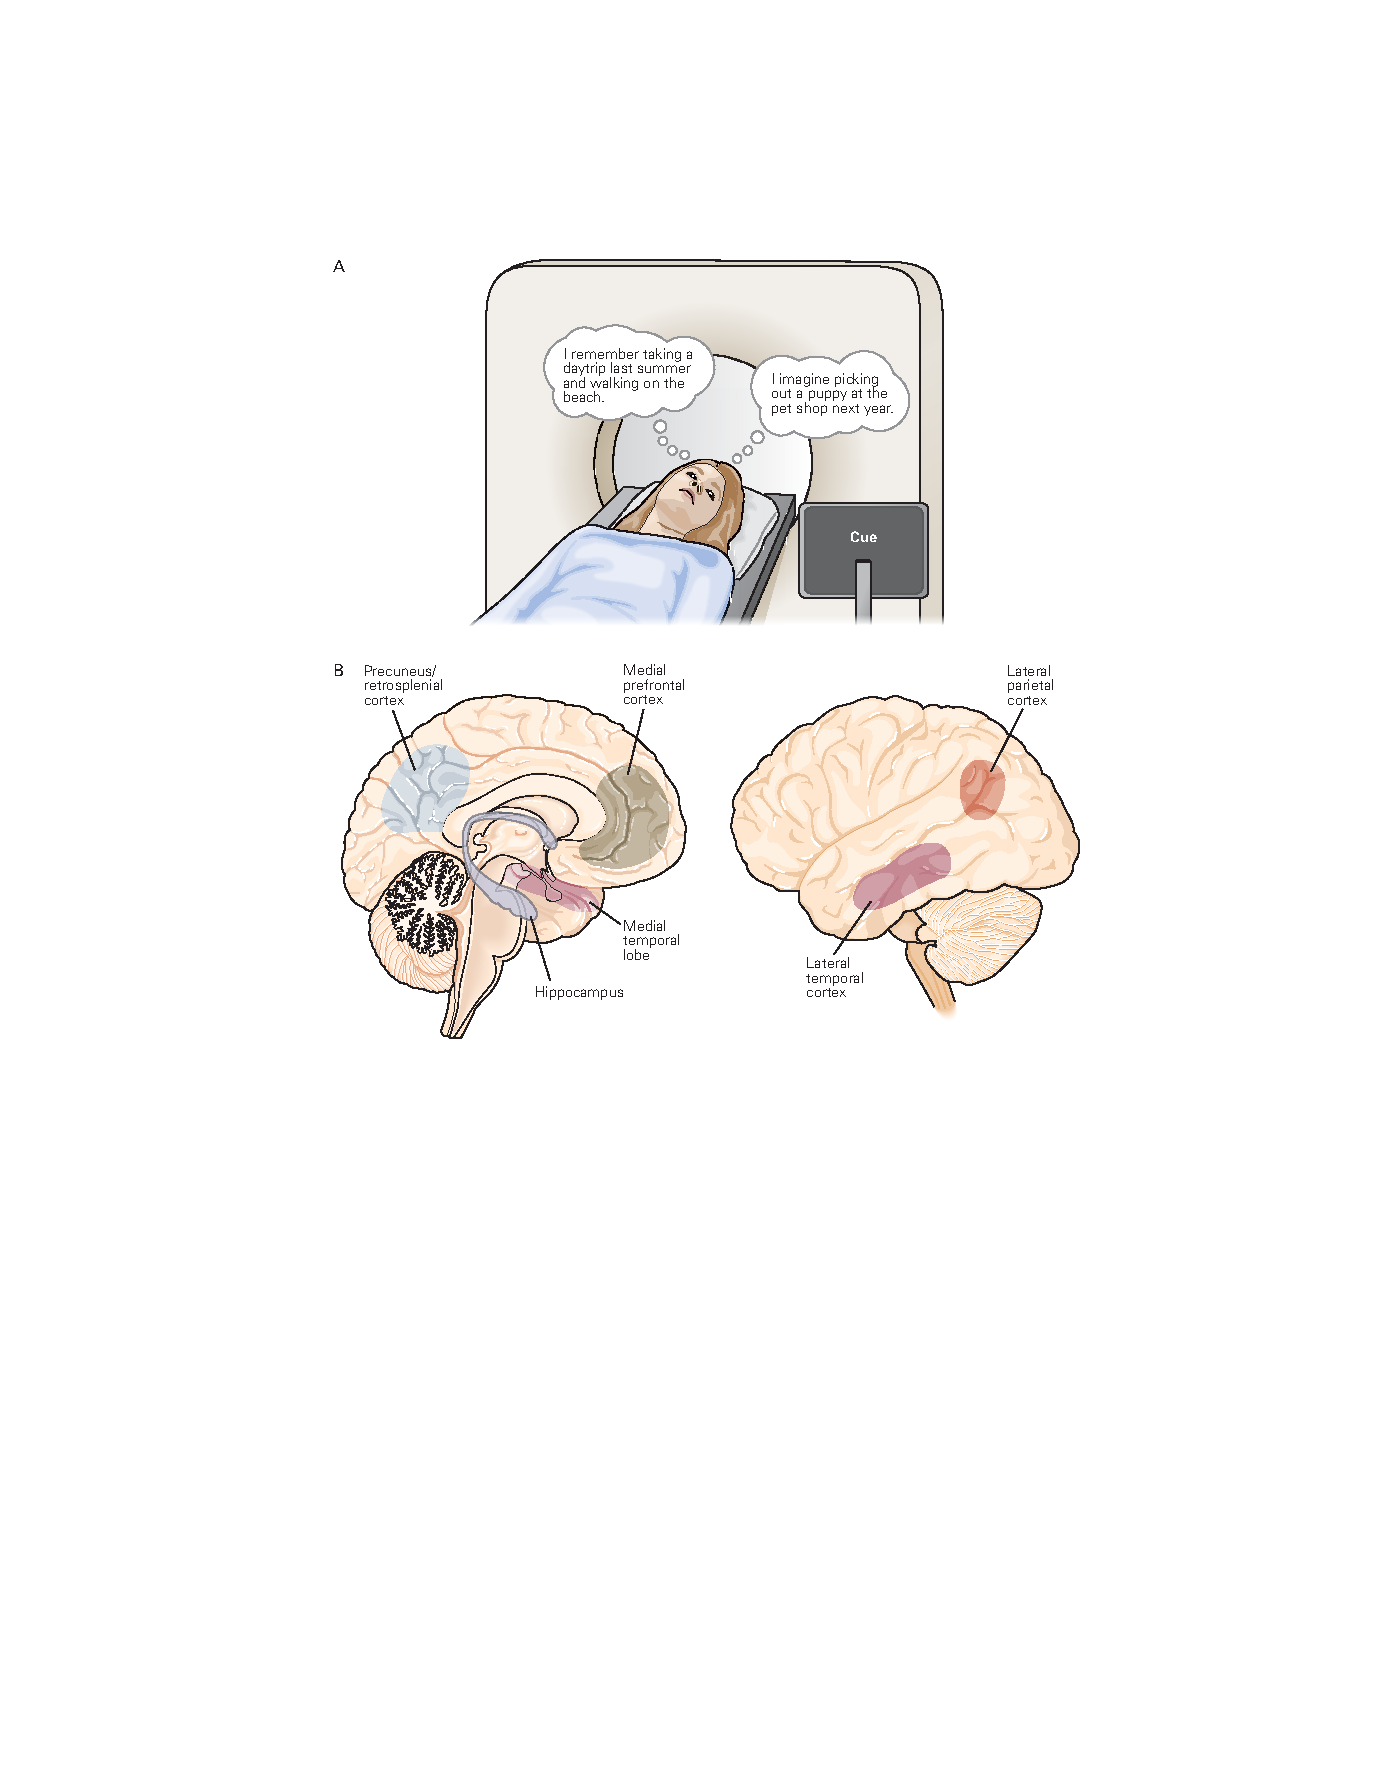
\includegraphics[width=0.87\linewidth]{chap52/fig_52_7}
	\caption{支持对过去事件的记忆检索和对未来事件的想象的大脑区域\cite{schacter2017episodic}。
		\textbf{A.} 受试者被要求在躺在功能性磁共振成像扫描仪中时回忆他们过去亲身经历的事件或想象他们未来可能发生的事件。
		事件由提示词(例如,“海滩”或“生日”)引发。
		事件现象学的主观评级(例如,情节的生动性和情感性)和详细的事件描述通常在扫描后的采访中获得,以确认情节事件已成功生成。
		\textbf{B.} 调解过去和未来思维的核心大脑系统在回忆过去、展望未来和进行相关形式的心理模拟时始终被激活。
		该网络的主要组成部分包括内侧前额叶区域、内侧和外侧顶叶皮层的后部区域(延伸到楔前叶和\textit{压后皮层})、外侧颞叶皮层和内侧颞叶。
		此外,这个核心大脑系统内的区域在功能上彼此相关,并与海马体相关。
		这个核心大脑系统被认为具有适应性功能,可以整合过去经验中有关关系和关联的信息,以构建关于未来可能事件的心理模拟。}
	\label{fig:52_7}
\end{figure}


支持情景记忆和海马体功能对于规划未来行为所必需的观点的进一步证据来自使用虚拟现实模拟对空间导航任务的人类表现的研究。
高分辨率\textit{功能性磁共振成像}和多体素模式分析(第~\ref{chap:chap6}~章)表明海马体的活动与导航目标的模拟有关。
此外,计划期间的海马体活动与前额叶、内侧颞叶和内侧顶叶皮层的目标相关活动共变(图~\ref{fig:52_8})。


\begin{figure}[htbp]
	\centering
	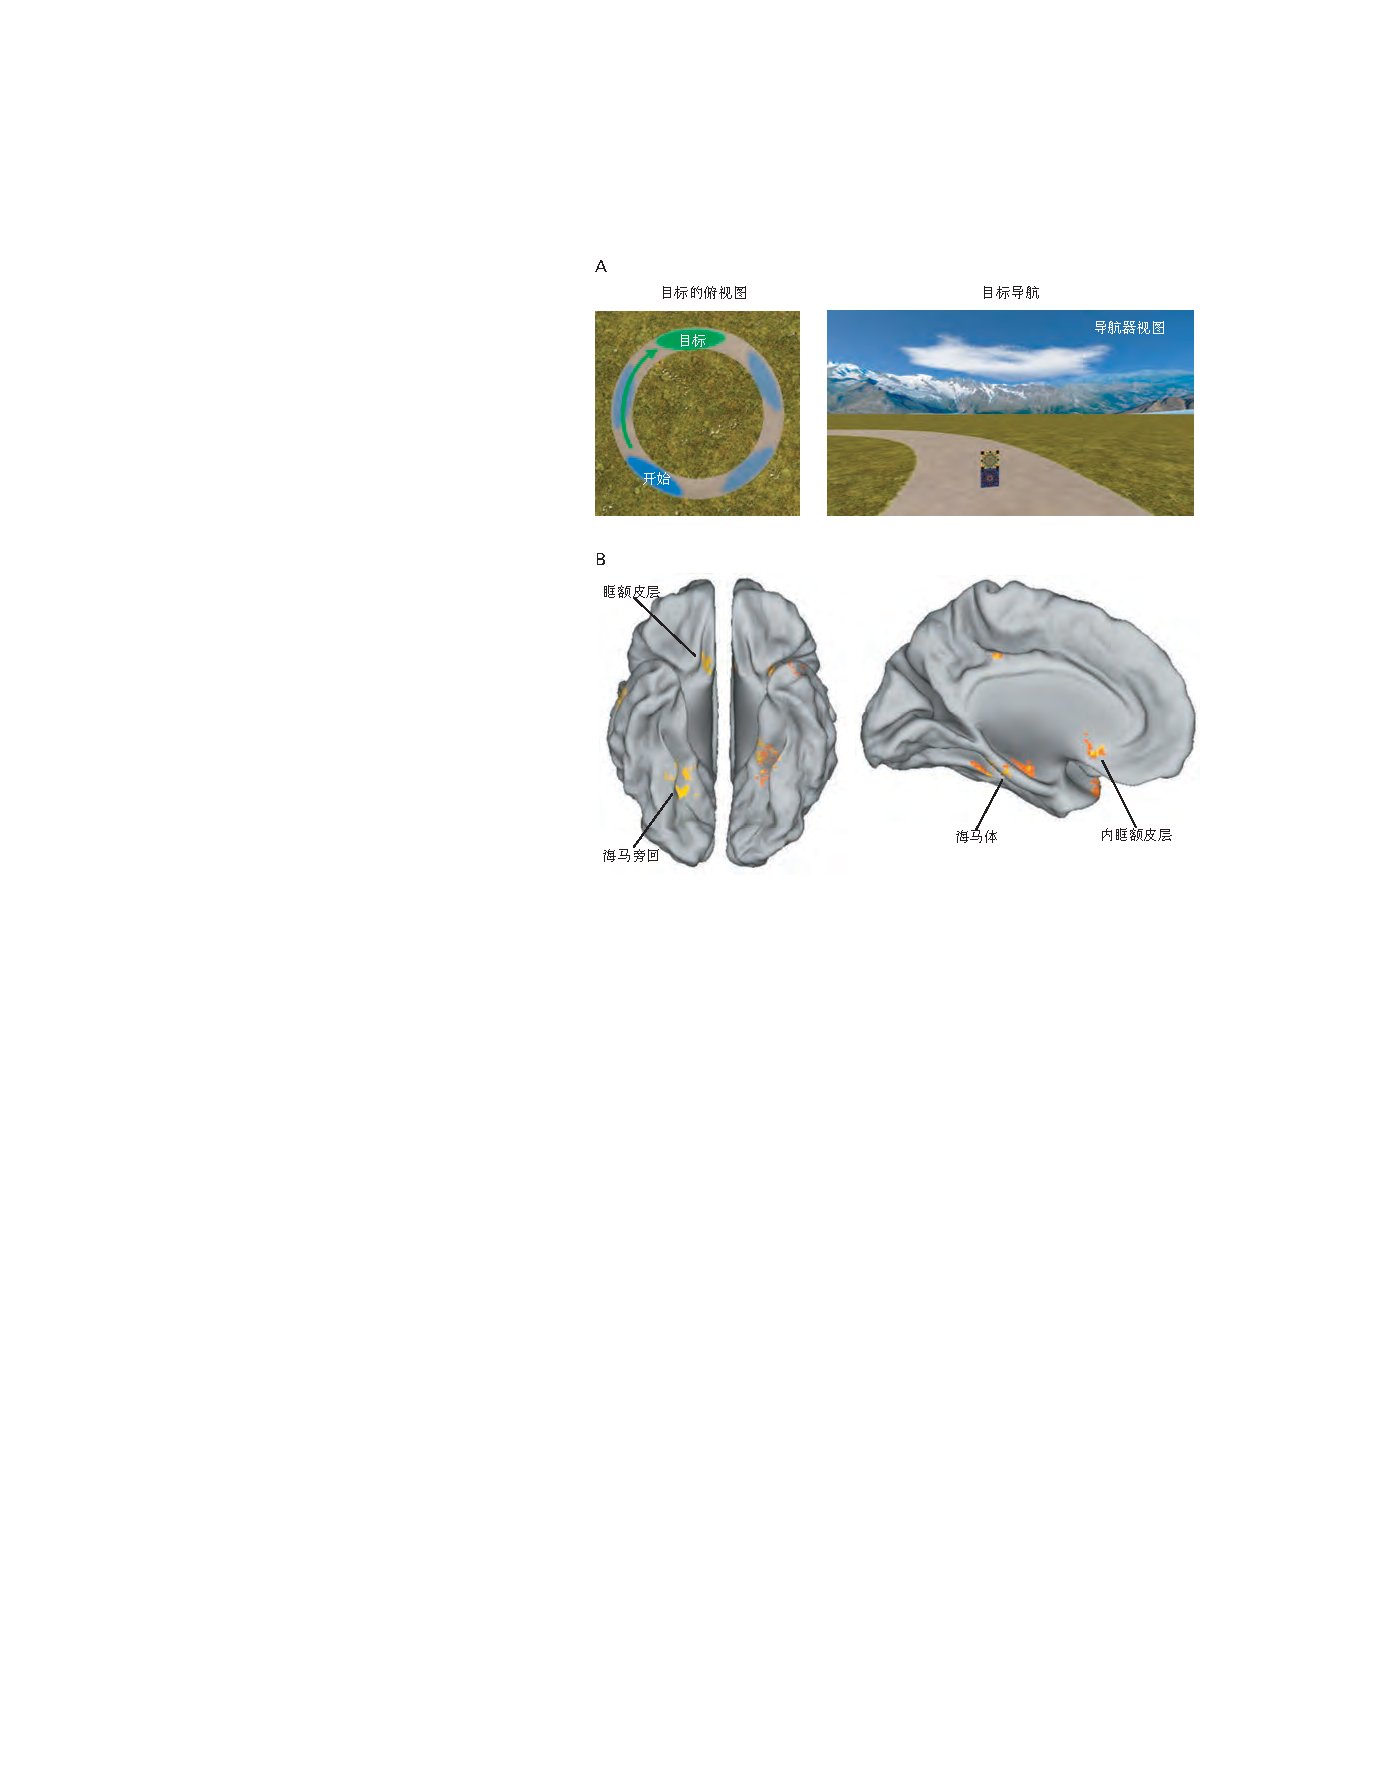
\includegraphics[width=0.78\linewidth]{chap52/fig_52_8}
	\caption{支持基于记忆的目标导向导航的神经回路\cite{brown2016prospective}。
		\textbf{A.} 人类参与者在使用功能性核磁共振成像进行扫描的同时,在虚拟现实环境中导航至目标。
		他们首先探索空间并了解目标所在的位置,然后测试他们导航到特定目标的能力。
		\textbf{B.} 导航规划在核心网络中引发与目标相关的活动,包括海马体、内侧颞叶、\textit{海马旁回}和\textit{眶额皮层}。}
	\label{fig:52_8}
\end{figure}


情景记忆的编码和存储也受到事件适应性价值的影响。
\textit{艾丽森$\cdot$阿德科克}及其同事表明,对潜在奖励的预期可以通过引发富含多巴胺神经元的内侧颞叶和中脑区域之间的协调活动来增强记忆力。
奖励也可以追溯增强记忆。
当人类参与者在迷宫中寻找奖励时,他们对奖励前发生的中性事件有更好的记忆。
根据结果追溯塑造情景记忆的能力很重要,因为特定事件的相关性可能只有在事后才知道。
连同情景记忆在构建过去事件的检索以及想象和模拟未来事件中的作用,关于奖赏的研究结果支持这样的观点,即情景记忆的主要功能是指导适应性行为。



\subsection{海马体通过建立关系关联来支持情景记忆}

除了海马体在情景记忆、未来思维和目标导向行为中的广泛作用外,对啮齿动物的研究首先指出了海马体在空间导航中的作用(第~\ref{chap:chap54}~章),这一发现后来得到了对非人类灵长类动物和人类的研究的支持。
在啮齿动物中,海马体中的单个神经元编码特定的空间信息,海马体的损伤会干扰动物的空间位置记忆。
健康人大脑的功能成像显示,当回忆空间信息时,右侧海马体的活动会增加,而当回忆单词、物体或人物时,左侧海马体的活动会增加。
这些生理学发现与临床观察结果一致,即右侧海马体的损伤不同地引起空间定向问题,而左侧海马体的损伤不同地导致言语记忆缺陷。


海马体支持空间处理、语义记忆和情景记忆这一事实引发了关于海马体如何促成这些不同行为的问题。
\textit{霍华德$\cdot$艾肯鲍姆}和\textit{尼尔$\cdot$科恩}提出的一个令人信服的理论表明,海马体提供了一种形成和存储复杂多模式关联的通用机制。
根据这种观点,海马体在记忆中结合了经验的独立元素,将事件编码为空间和时间上下文中项目的关系图,从而构成了一个“记忆空间”,可以区分不同的情节或事件序列,即使当相同(或相似)的事件发生在不同的情节中(图~\ref{fig:52_9})。
正如本章后面所讨论的,海马体编码关系的观点提供了对记忆建立机制的见解,并解释了为什么在某些情况下,海马体可能有助于无法有意识地访问但确实编码关系的记忆过程。


\begin{figure}[htbp]
	\centering
	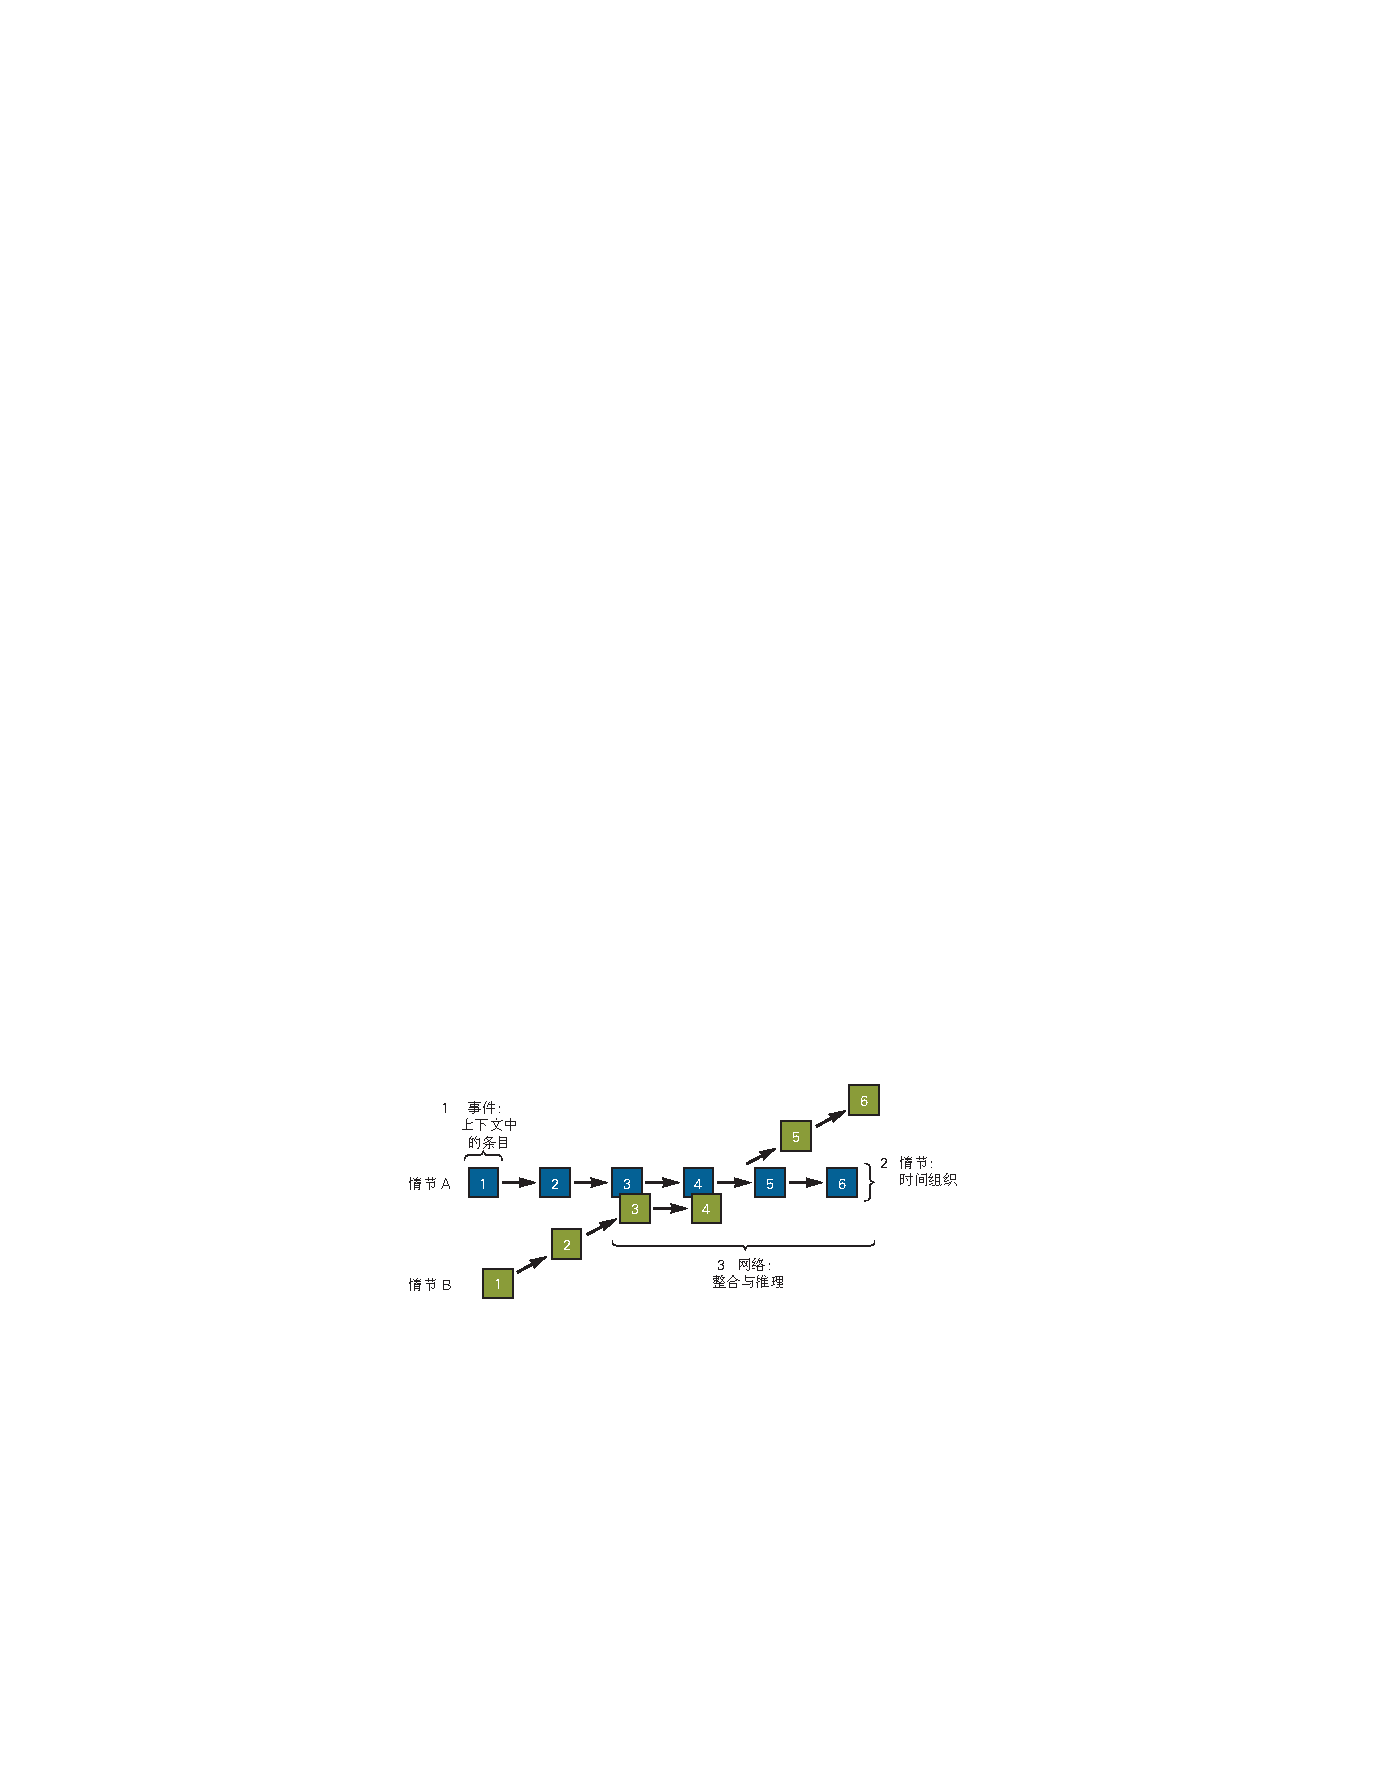
\includegraphics[width=0.8\linewidth]{chap52/fig_52_9}
	\caption{海马体支持情景记忆的相关处理。
		记忆空间的概念图,指定三种关键类型的关系处理:\textit{事件}、\textit{情节}和\textit{网络}。
		该示意图说明了两个不同情节(情节 A 和情节 B)的处理,它们具有不同和重叠的元素。
		例如,情节可能是在不同的晚上与同一个朋友两次不同地访问一家意大利餐馆。
		晚上的经历是截然不同的(不同的日子、不同的天气、不同的心情),但它们也有一些重叠(同一家餐厅的同一位朋友的陪伴)。
		事件(1)被定义为与其发生的上下文相关联的项目(对象、行为)(此处表示为每个情节中的事件 1 到 6,例如您坐在的特定桌子、您订购的食物等)。
		情节(2)在这个观点中被定义为这些事件的时间组织。 虽然每一集中的大多数项目都是独一无二的,但其中一些是重叠的(此处为项目 3 和 4;在示例中为您的朋友和餐厅)。
		关系网络(3)是通过重叠事件通过事件和情节之间的关联形成的,支持间接相关事件之间的链接能力\cite{eichenbaum2014can}。 }
	\label{fig:52_9}
\end{figure}



\section{内隐记忆支持人类和动物的一系列行为}

正如外显记忆以多种方式引导行为一样,非外显形式的记忆(那些没有意识的记忆)也可以通过多种方式影响行为。
内隐记忆是指在没有意识的情况下指导行为的知识形式。
例如,启动是暴露于一个提示对处理后续提示的自动影响。


启动可分为概念启动或知觉启动。
概念启动提供了对与任务相关的语义知识的增强访问,因为以前已经使用过该知识。
它与有助于语义知识初始检索的左前额叶区域活动减少相关。
相比之下,知觉启动发生在特定的感觉形态中,并依赖于皮层模块,这些模块根据关于单词和物体的形式和结构的感觉信息进行操作。


皮层单峰感觉区域的损伤会损害特定模态的知觉启动。
例如,一名右枕叶有广泛手术损伤的患者未能表现出对单词的视觉启动,但具有正常的外显记忆(图~\ref{fig:52_10})。
这种情况与在叫\textit{亨利$\cdot$莫莱森}等健忘症患者中发现的情况相反,表明启动的神经机制与外显记忆的神经机制不同。
由于内侧颞叶损伤导致的健忘症患者的知觉启动可能完好无损,这一事实进一步表明它与外显记忆不同。


\begin{figure}[htbp]
	\centering
	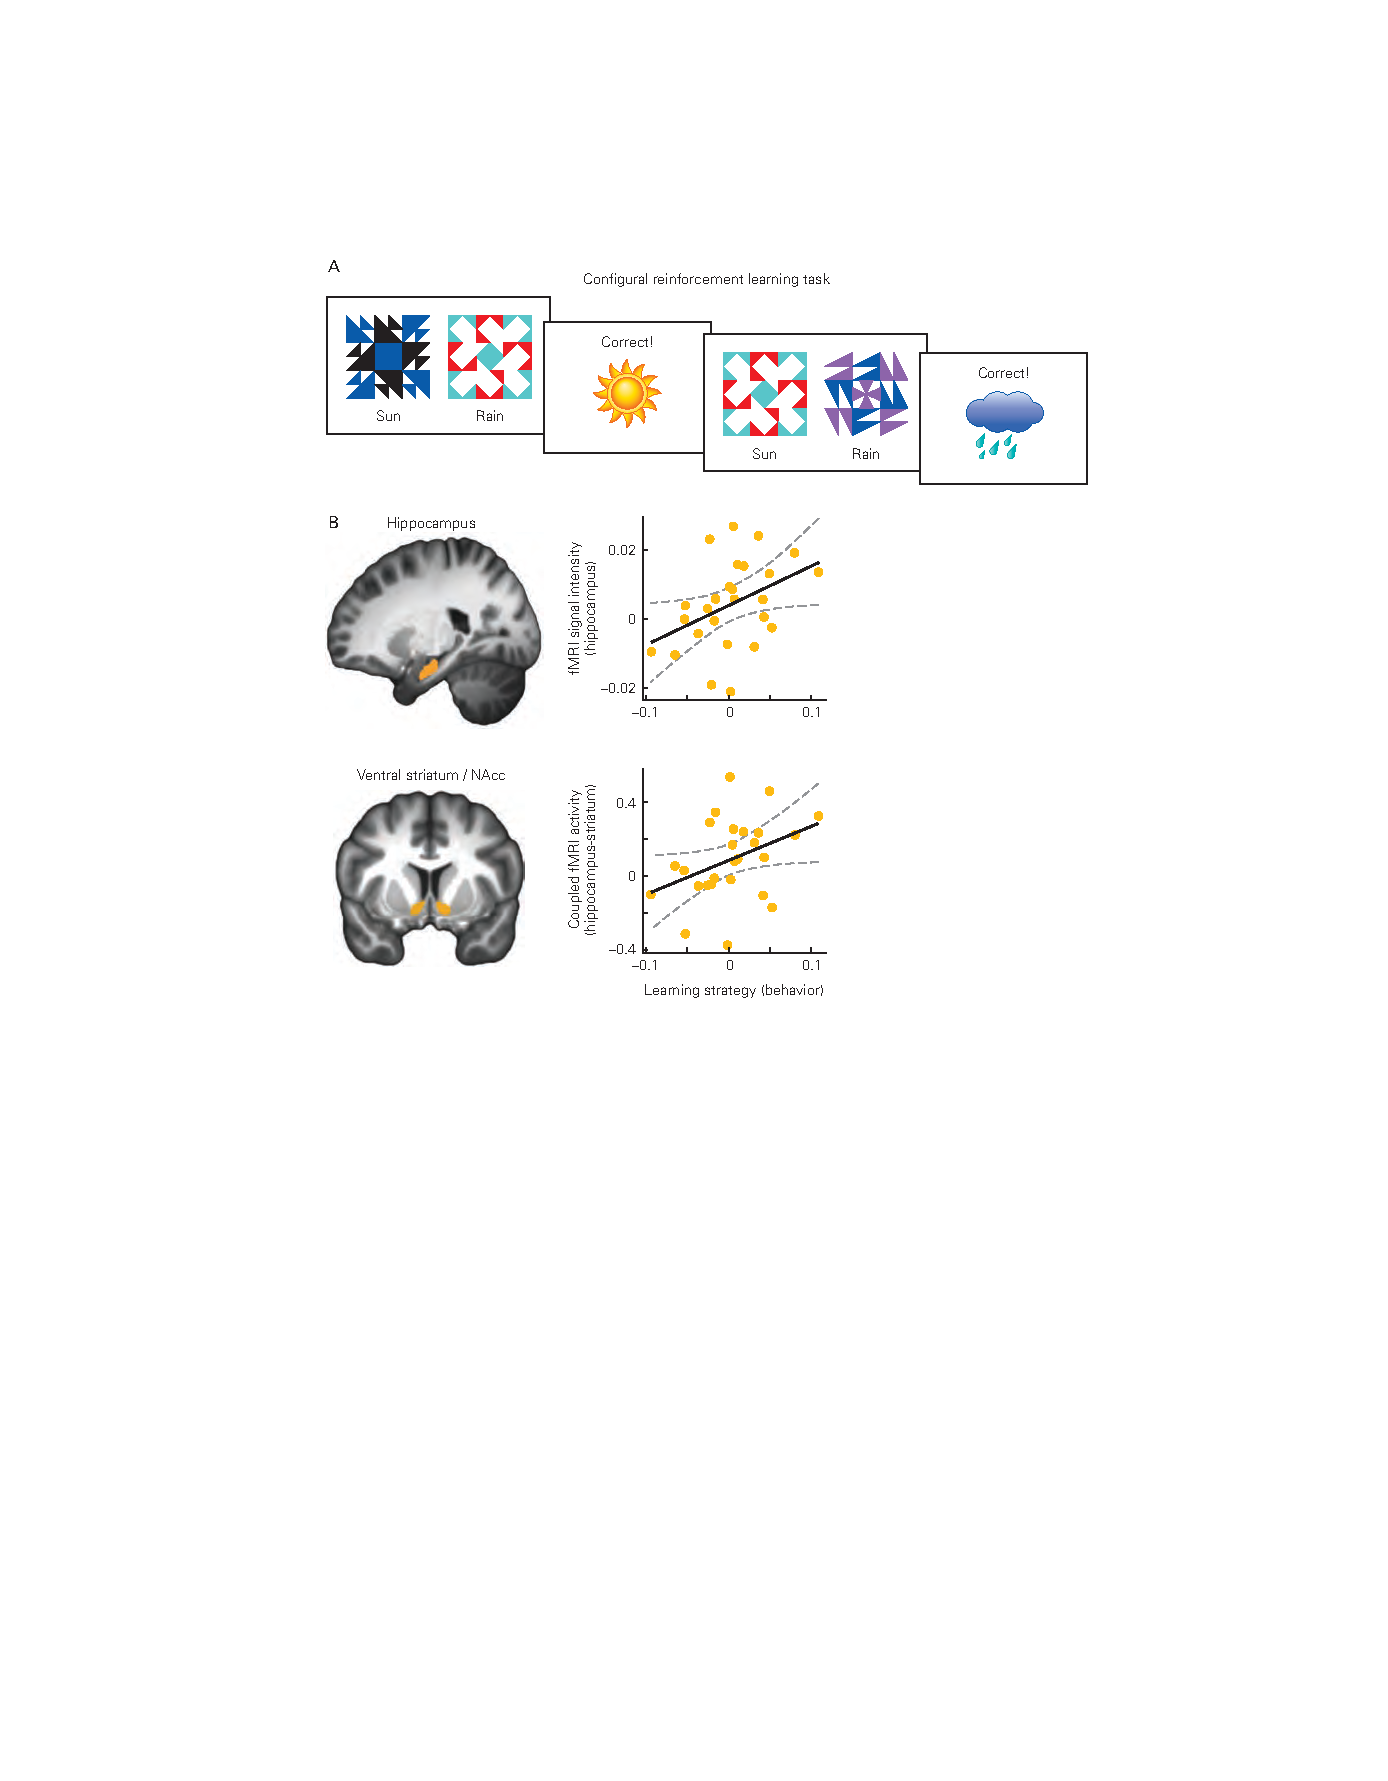
\includegraphics[width=0.92\linewidth]{chap52/fig_52_10}
	\caption{单词的视觉启动需要右枕叶皮层\cite{vaidya1998font}。
		\textbf{A.} 结构磁共振成像显示患者 M.S. 的右枕骨皮层几乎完全切除,该患者患有药理学上顽固性癫痫,右侧枕骨皮质病灶。
		\textbf{B.} 字体特定启动是视觉启动的一种形式,与字体不同时的识别相比,当字体与早期呈现相同时,个人能够更好地识别短暂闪烁的单词。
		启动的衡量标准是字体相同时的性能减去字体不同时的性能。
		字体特异性启动在\textit{失忆症患者}及其对照以及患者 M.S. 的对照中是完整的,但在 M.S. 他自己中则不然。
		病人 M.S. 具有正常的外显记忆,甚至对于视觉提示(数据未显示),但缺乏对视觉呈现的单词的特定属性的内隐记忆。}
	\label{fig:52_10}
\end{figure}



\subsection{不同形式的隐式记忆涉及不同的神经回路}

其他形式的内隐记忆有助于习惯和运动、知觉和认知技能的学习,以及条件反应的形成和表达。
一般来说,这些形式的内隐记忆的特点是增量学习,随着重复逐渐进行,在某些情况下,是由强化驱动的。


习惯、运动技能和条件反应的学习可以独立于内侧颞叶系统进行。
例如,叫\textit{亨利$\cdot$莫莱森}能够获得新的视觉运动技能,如镜像追踪任务(见图~\ref{fig:52_3})。
因此,早期的理论认为这些形式的记忆通常不依赖于内侧颞叶,而是依赖于基底神经节和小脑(见第~\ref{chap:chap37}~和~\ref{chap:chap38}~章)。
然而,随后的研究表明,这不是一般规则,内侧颞叶是存储关系关联的内隐学习形式所必需的,即使这种关联是通过重复学习的,并且似乎是在没有意识的情况下发生的。


现在认为有几种增量内隐学习涉及内侧颞叶。
例如,\textit{图尔克$\cdot$布朗}及其同事研究了\textit{视觉提示}之间规律性的内隐学习,称为统计学习。
在典型的统计学习任务中,人类受试者会收到一系列声音或图像,这些声音或图像遵循结构化序列或重复的“语法”。
序列的学习通常通过与非重复序列相比对重复序列更快的反应时间来衡量。
乍一看,统计学习似乎不应该涉及内侧颞叶:
学习是非语言的,不需要有意识的思考,因此是隐含的,并且假设它反映了跨多个事件的概率关系的累积计算,而不是某一集的具体记忆。
然而,\textit{功能性核磁共振成像}研究表明,海马体在统计学习过程中是活跃的,并且已经发现内侧颞叶的损伤会损害这项隐性任务的表现。


统计学习是学习如何通过重复发生的一个例子。
新的感知、运动或认知能力也通过重复学习。
通过练习,性能变得更准确、更快,并且这些改进可以推广到学习新信息。
技能学习从认知阶段转移到自主阶段,在认知阶段知识被明确表示,学习者必须非常注意表现,自主阶段可以在没有太多有意识的关注的情况下执行技能。
例如,驾驶汽车最初需要有意识地了解技能的每个组成部分,但在练习之后,人们不再关注各个组成部分。


感觉运动技能的学习取决于许多大脑区域,这些区域随着所学习的特定关联而变化。
正如我们在第~\ref{chap:chap38}~章中了解到的,这些包括基底神经节、小脑和新皮层。
帕金森病和亨廷顿病患者的基底神经节功能障碍会影响运动技能的学习。
患有小脑病变的患者也难以获得一些运动技能。
健康个体在感觉运动学习过程中的功能成像显示基底神经节和小脑的活动及其与皮层区域的连接发生变化。
\textit{丹妮尔$\cdot$巴西特}及其同事使用应用于全脑功能性核磁共振成像数据的网络分析算法来表征在运动技能学习期间发生的网络功能连接的动态变化。
最后,熟练的行为可能取决于运动新皮层的结构变化,如音乐家手指的皮层表征的扩展所示(第~\ref{chap:chap53}~章)。


习惯是从提示或行动与奖励结果的反复关联中产生的。
人类的习惯学习是通过涉及刺激-奖励关联的增量学习的任务来研究的。
在一项典型的任务中,受试者会进行一系列试验,要求他们在视觉提示中进行选择,并逐个试验地接受有关他们选择的反馈。
提示和反馈之间的关系在任务过程中可能会发生变化,因此参与者必须根据反馈不断更新他们的反应。
因为学习是在多次试验中进行的,所以对任何一个特定试验的明确记忆对于成功的表现可能不如逐渐积累刺激-结果关联的反馈驱动学习那么有用。


\textit{功能性磁共振成像}研究表明,刺激-奖励关联的增量学习取决于纹状体,即接收来自新皮层输入的基底神经节区域及其调节性多巴胺能输入。
纹状体多巴胺缺失的患者,如帕金森病患者,在逐项强化试验的基础上学习效果较差。
这些发现与其他研究一致,表明多巴胺在调节强化学习的皮层-纹状体回路中具有重要作用(见第~\ref{chap:chap38}~章)。


乍一看,刺激奖赏学习似乎恰恰是一种不依赖于内侧颞叶的学习:它是隐性的而不是显性的,它是逐渐发生的而不是通过对单个事件的显性记忆。
事实上,早期的理论假设学习概率刺激-奖励关联并不依赖于内侧颞叶。
然而,随后的工作表明,在某些情况下,海马体确实有助于刺激-奖励学习,例如当任务需要学习更复杂的刺激-刺激关联时(图~\ref{fig:52_11})。
海马体对内隐学习的贡献是通过与其他皮层和皮层下回路的相互作用发生的。
\textit{功能性磁共振成像}研究显示海马体和纹状体之间的功能连接支持跨各种任务的学习。
海马体和纹状体之间的相互作用有时是竞争性的,有时是合作性的,这取决于任务的要求。


\begin{figure}[htbp]
	\centering
	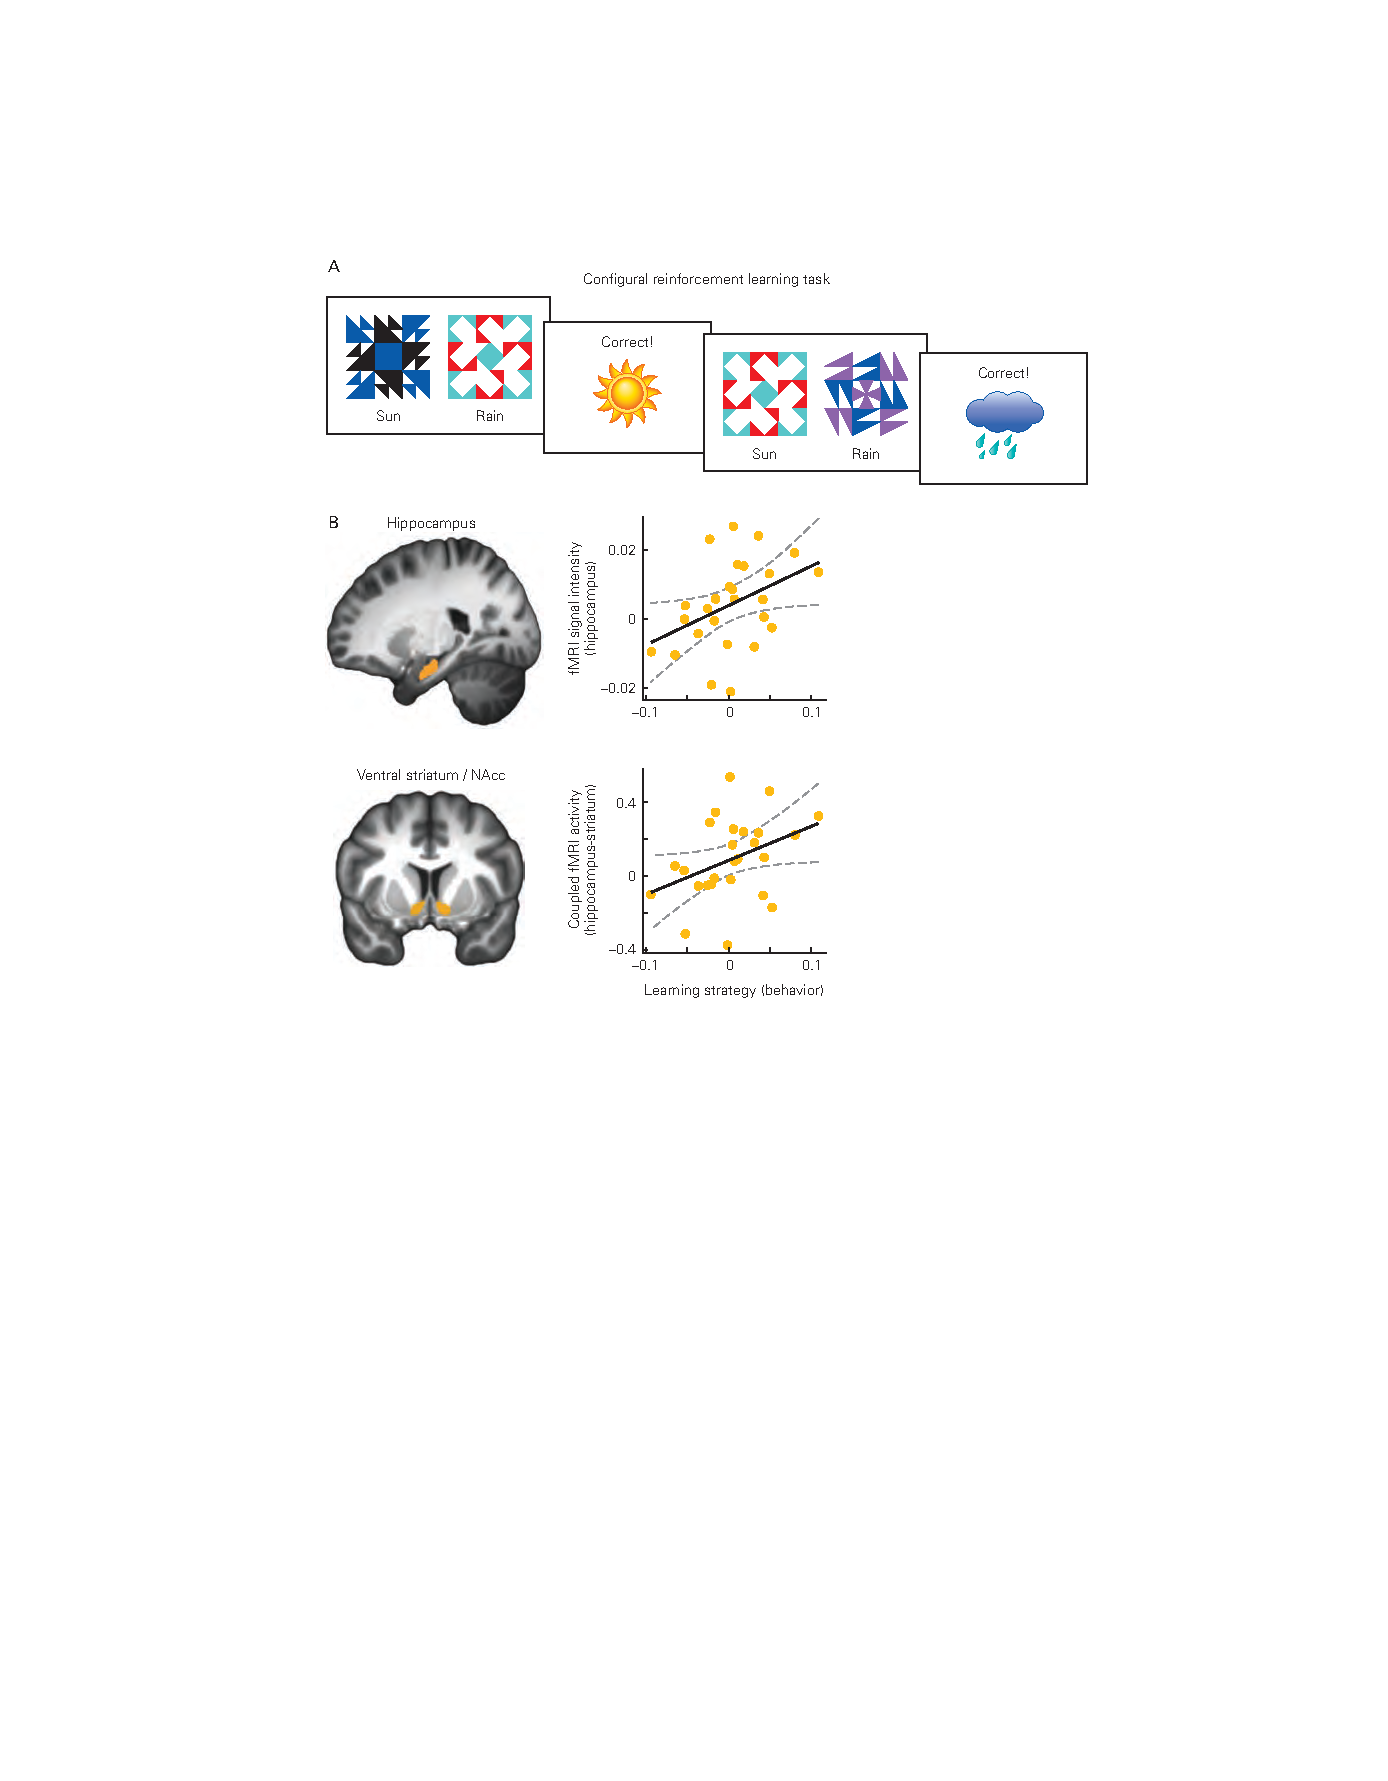
\includegraphics[width=0.92\linewidth]{chap52/fig_52_11}
	\caption{学习刺激-反应关联涉及纹状体和海马体\cite{duncan2018more}。
		\textbf{A.} 参与者通过试验强化来学习根据提示(彩色形状)预测结果(下雨或太阳)。
		这些提示与观众通过反复试验获悉的每种天气结果具有概率关系。
		可以根据每个单独的提示或两个提示的组合呈现(它们的配置)来预测天气。
		强化学习模型可以辨别每个主题使用哪种策略。
		\textbf{B.} 众所周知,纹状体在学习基于强化更新选择方面发挥着关键作用。
		当受试者了解配置时,同样的任务也会引起海马体的活动,并增加海马体和纹状体活动的耦合。
		散点图显示受试者使用配置学习策略的程度与海马体中血氧水平依赖性活动以及海马体和纹状体之间的功能耦合相关。
		这些图像显示了海马体和\textit{伏隔核}的活动,伏隔核是纹状体腹侧的一个区域,对奖赏刺激做出反应。}
	\label{fig:52_11}
\end{figure}



\subsection{内隐记忆可以是关联的或非关联的}

一些形式的内隐记忆也在非人类动物身上进行了研究,这些动物研究区分了两种类型的内隐记忆:非联想和联想。
通过非联想学习,动物可以了解单一刺激的特性。
通过联想学习,动物可以了解两种刺激之间或刺激与行为之间的关系。
我们将在下一章考虑动物内隐记忆的细胞机制。


当受试者一次或多次暴露于单一类型的刺激时,就会产生非联想学习。
两种形式的非联想学习在日常生活中很常见:习惯化和敏感化。
习惯化是当反复出现良性刺激时发生的反应减少。
例如,大多数美国人在独立日第一次听到鞭炮声时会感到吃惊,但随着时间的推移,他们会习惯这种噪音而不会做出反应。
敏化(或伪条件反射)是在呈现强烈或有害刺激后对各种刺激的增强反应。
例如,动物在受到痛苦的挤压后会对轻微的触觉刺激做出更强烈的反应。
此外,敏化刺激可以超越习惯化的影响,这一过程称为去习惯化。
例如,在习惯化减少了对噪音的惊吓反应后,可以通过用力捏一下来恢复对噪音的反应强度。


对于致敏和去习惯,刺激的时间并不重要,因为不必了解刺激之间的关联。
相反,对于两种形式的联想学习,关联刺激的时机至关重要。
经典条件反射涉及学习两种刺激之间的关系,而操作条件反射涉及学习有机体行为与该行为的后果之间的关系。


俄罗斯生理学家\textit{伊万$\cdot$巴甫洛夫}在 1900 年代初首次描述了经典条件反射。
经典条件反射的本质是两种刺激的配对:条件刺激和非条件刺激。
选择\textit{条件刺激},例如光、音调或触摸,是因为它不会产生明显的反应或通常与最终将学会的反应无关的微弱反应。
选择\textit{非条件刺激},例如食物或电击,因为它通常会产生强烈且一致的反应(无条件反应),例如流涎或缩回肢体。
无条件的反应是天生的;
它们是在没有学习的情况下产生的。
在\textit{非条件刺激}之后重复呈现\textit{条件刺激}会逐渐引发一种新的或不同的反应,称为条件反应。


一种解释条件作用的方法是,\textit{条件刺激}和\textit{非条件刺激}的重复配对导致\textit{条件刺激}成为\textit{非条件刺激}的预期信号。
有了足够的经验,动物会对\textit{条件刺激}做出反应,就好像它在期待\textit{非条件刺激}一样。
例如,如果一盏灯之后反复出现肉,最终看到灯本身就会使动物垂涎三尺。
因此,经典条件反射是动物学习预测事件的一种方式。


如果在没有\textit{非条件刺激}的情况下重复呈现\textit{条件刺激},则已建立的条件反应发生的可能性会降低。
这个过程被称为灭绝。
如果与食物配对的光后来在没有食物的情况下反复出现,它会逐渐停止引起流涎。
灭绝是一种重要的适应机制;
动物继续对不再有意义的线索做出反应是不适应的。
现有证据表明,灭绝与遗忘不同;
相反,学到了一些新东西,\textit{条件刺激}现在发出美国不会出现的信号。


多年来,心理学家认为只要\textit{条件刺激}在关键时间间隔内先于\textit{非条件刺激},就会产生经典条件反射。
根据这种观点,每当\textit{条件刺激}后面跟着 \textit{非条件刺激}(强化刺激)时,刺激和反应的内部表征之间或一种刺激和另一种刺激的表征之间的联系就会得到加强。
连接的强度被认为取决于\textit{条件刺激}和\textit{非条件刺激}的配对数量。
现在大量证据表明,经典条件反射不能简单地用两个事件或刺激相继发生这一事实来充分解释(图~\ref{fig:52_12})。
事实上,仅仅依赖顺序是不适应的。
相反,所有能够进行联想调节的动物,从蜗牛到人类,都记得关联事件之间的显著关系。
因此,经典条件作用,或许还有所有形式的联想学习,使动物能够区分可靠地一起发生的事件和那些只是随机关联的事件。


\begin{figure}[htbp]
	\centering
	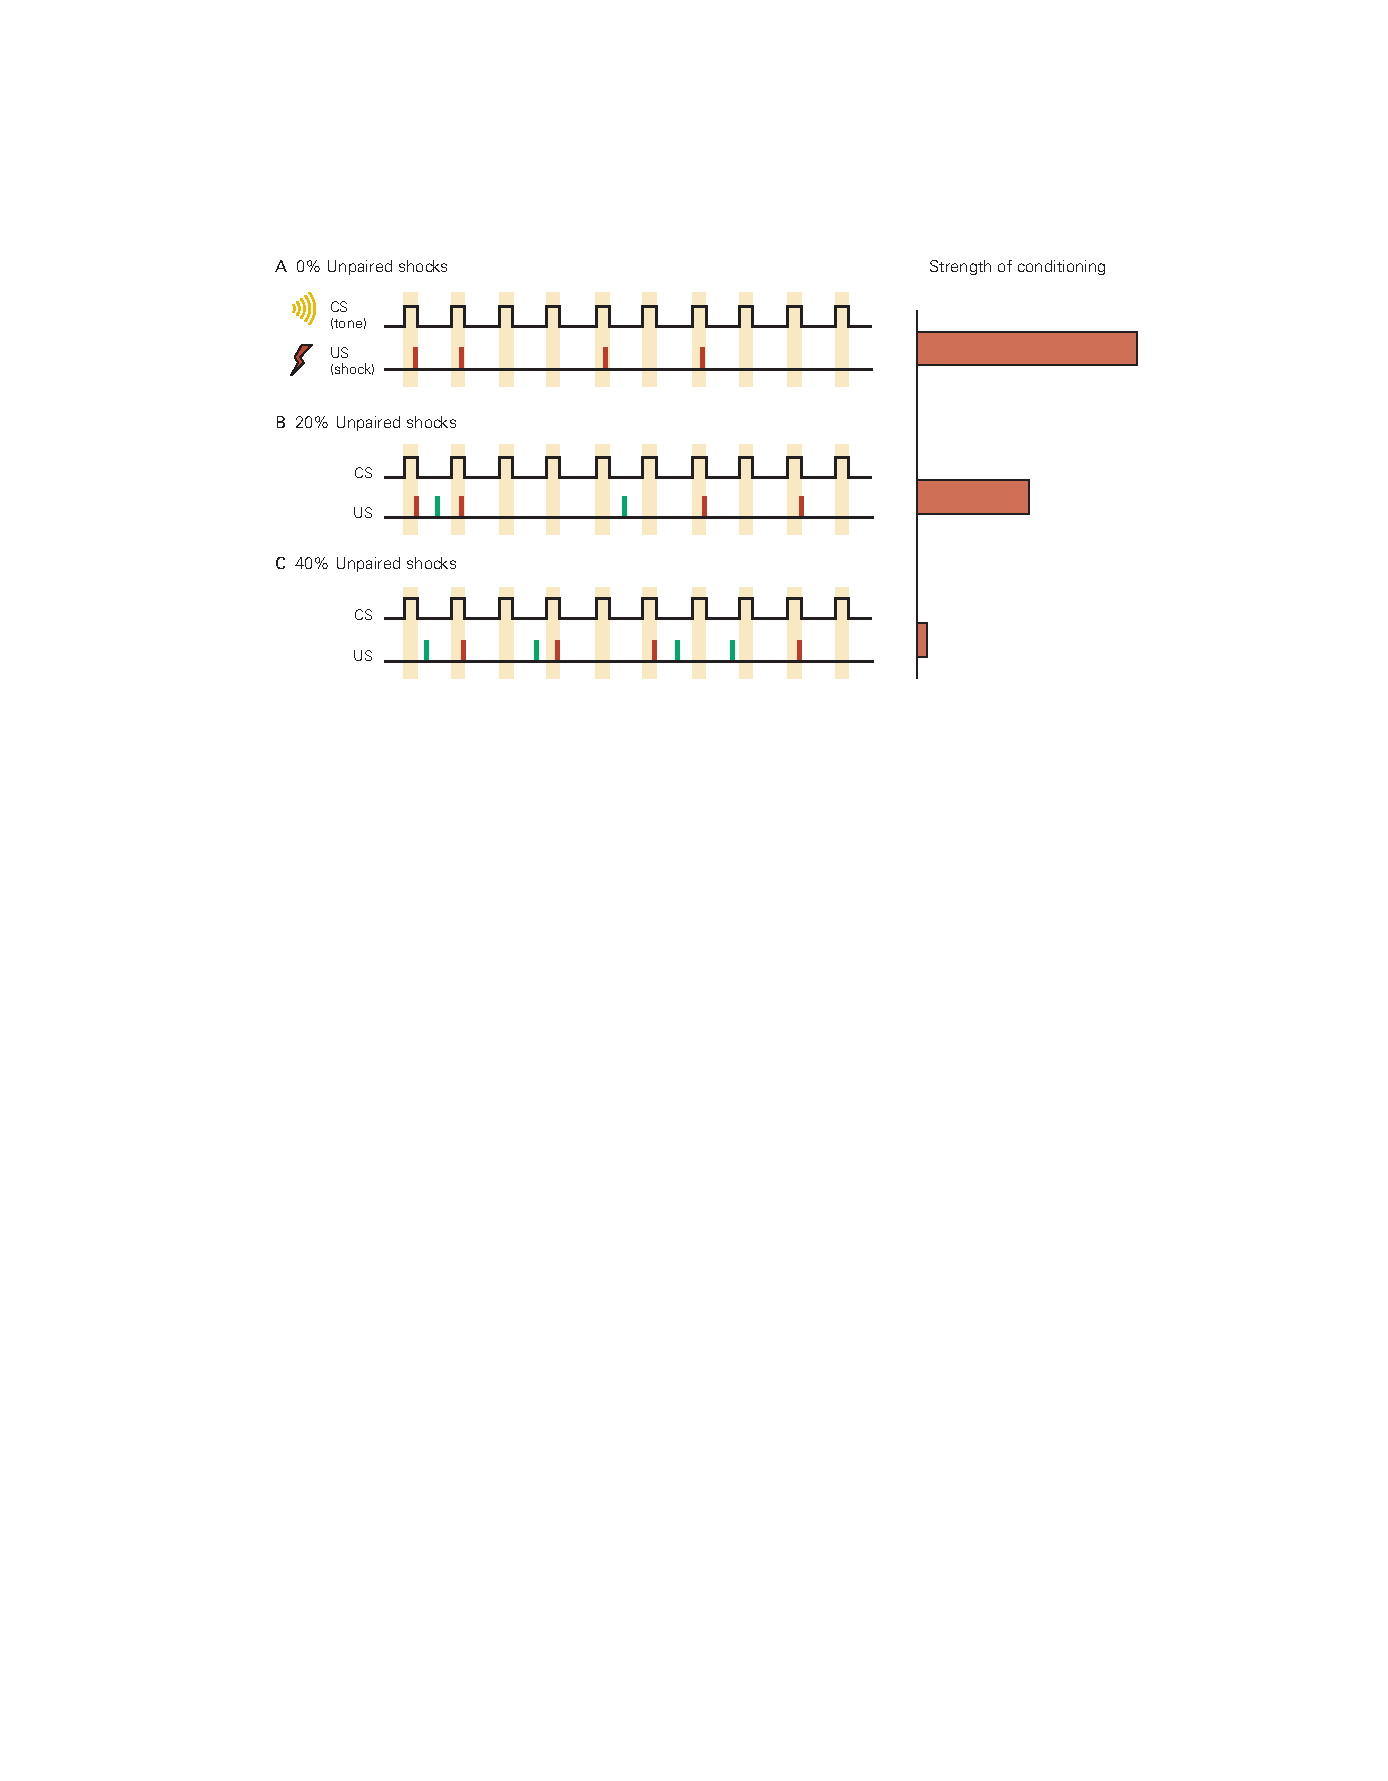
\includegraphics[width=0.98\linewidth]{chap52/fig_52_12}
	\caption{经典条件反射取决于两个刺激的相关程度。
		在这项针对大鼠的实验中,在 10 项试验中有 4 项(红色勾号)将音调(\textit{条件刺激})与电击(\textit{非条件刺激})配对。
		在某些试验块中,电击是在没有音调(绿色勾号)的情况下呈现的。
		抑制杠杆获取食物是冻结的标志,这是一种有条件的防御反应。
		通过确定仅音调在抑制杠杆按压以获得食物方面的效果来评估调节的程度\cite{rescorla1968probability}。
		\textbf{A.} 当美国只接受\textit{条件刺激}时,会出现最大条件反射。 
		当没有音调出现电击时几乎和有音调时一样频繁地出现(40\%),很少或没有条件反射。
		当 20\% 的时间没有音调发生电击时,就会发生一些条件反射。}
	\label{fig:52_12}
\end{figure}


大脑多个区域的损伤会影响经典条件反射。
一个经过充分研究的例子是保护性眨眼反射的调节,这是一种运动学习形式。
一股空气吹到眼睛自然会引起眨眼。
可以通过将粉扑与粉扑之前的音调配对来建立有条件的眨眼。
对兔子的研究表明,条件反应(对音调的眨眼反应)会被两个部位中任一处的损伤所消除。
对\textit{小脑蚓体}的损伤会消除条件反应,但不会影响非条件反应(眨眼以响应一股空气)。
有趣的是,小脑同一区域的神经元表现出依赖于学习的活动增加,这与条件行为的发展密切相关。
小脑深部核\textit{间位核}的损伤也会消除条件性眨眼。
因此,\textit{小脑蚓体}和深部核团在调节眨眼以及涉及骨骼肌运动的其他简单形式的经典调节中都起着重要作用。


另一个经过充分研究的例子是恐惧条件反射,它取决于杏仁核。
在恐惧条件反射中,中性提示(例如语气)与令人厌恶的结果(例如震惊)配对。
这种配对会导致条件性恐惧反应,其中中性语气会单独引发行为反应,例如冻结。
恐惧条件反射取决于杏仁核亚核输入和连接的可塑性,尤其是基底外侧杏仁核,我们将在下一章讨论。



\subsection{操作性条件反射涉及将特定行为与强化事件相关联}

由\textit{桑代克}发现并由\textit{斯金纳}等人系统研究的联想学习的第二个主要范例是操作条件反射(也称为试错学习)。
在操作性条件反射的典型实验室示例中,一只饥饿的老鼠或鸽子被放置在一个试验室中,在该试验室中动物会因特定行为而获得奖励。
例如,腔室可具有从一个壁突出的杠杆。 由于之前的学习,或通过玩耍和随机活动,动物会偶尔按下杠杆。
如果动物在按下杠杆后立即接受正强化物(例如,食物),它将开始比自发率更频繁地按下杠杆。
动物可以被描述为已经学会在它的许多行为(例如,梳理、饲养和行走)中,一种行为之后是食物。
有了这些信息,动物很可能会在饥饿时按下控制杆。


如果我们将经典条件反射视为两种刺激(\textit{条件刺激}和\textit{非条件刺激})之间预测关系的形成,则操作性条件反射可被视为行动与结果之间预测关系的形成。
与测试反射对刺激的反应性的经典条件反射不同,操作性条件反射测试自发发生或没有可识别刺激的行为。
因此,据说操作性行为是发出的而不是引发的。
一般来说,获得奖励的行为往往会被重复,而伴随着厌恶行为的行为虽然不一定是痛苦的,但其后果往往不会重复。
许多实验心理学家认为,这个被称为效果法则的简单概念支配着许多自愿行为。


操作性条件反射和经典条件反射涉及不同类型的关联,分别是动作与奖励之间或两种刺激之间的关联。
然而,操作性条件反射和经典条件反射的规律非常相似。
例如,时机对两者都至关重要。
在操作性条件反射中,强化物通常必须紧跟操作性动作。
如果强化剂延迟太久,只会发生弱调节。
同样,如果\textit{条件刺激}和\textit{非条件刺激}之间的间隔太长或者如果\textit{非条件刺激}在\textit{条件刺激}之前,则经典调节通常很差。



\subsection{联想学习受到生物体生物学的限制}

动物通常学会将与其生存相关的刺激联系起来。
例如,动物很容易学会避免某些食物,这些食物随后会产生负强化(例如,毒药引起的恶心),这种现象称为味觉厌恶。


与大多数其他形式的条件反射不同,即使在长时间延迟后发生非条件反应(毒物引起的恶心)时,味觉厌恶也会发生,直到\textit{条件刺激}(特定味道)后数小时。
这在生物学上是有道理的,因为受感染的食物和天然产生的毒素的不良影响通常是在经过一段时间的摄入后才产生的。
对于包括人类在内的大多数物种,只有当某些口味与疾病相关时才会发生味觉厌恶调节。
如果味觉之后是不产生恶心的痛苦刺激,则味觉厌恶发展不佳。
此外,动物不会对伴随恶心的视觉或听觉刺激产生厌恶。



\section{记忆中的错误和缺陷揭示了正常的记忆过程}

记忆让我们重温个人的过去; 提供对事实、关联和概念的庞大网络的访问; 并支持学习和适应行为。 但记忆并不完美。
我们经常会迅速或逐渐忘记事件,有时会扭曲过去,偶尔会记住我们宁愿忘记的事件。
在 1930 年代,英国心理学家\textit{弗雷德里克$\cdot$巴特莱特}报告了人们阅读并试图记住复杂故事的实验。
他表明,人们经常会记错故事的许多特征,经常会根据他们对本应发生的事情的预期来歪曲信息。
遗忘和扭曲可以提供对记忆运作的重要见解。


记忆的缺陷被分为七个基本类别,被称为“记忆的七大罪”:\textit{稍纵即逝}、\textit{心不在焉}、\textit{阻塞}、\textit{错误归因}、\textit{易受暗示}、\textit{偏见}和不受欢迎的\textit{纠缠}。
在这里,我们重点关注其中的六个。


\textit{心不在焉}是由于缺乏对直接经验的关注。
编码过程中的注意力不集中可能是常见记忆失败的根源,例如忘记最近放置目标的位置。
当我们忘记执行某项特定任务(例如在从办公室回家的路上买杂货)时,也会出现心不在焉,即使我们最初对相关信息进行了编码。


\textit{阻塞}是指暂时无法访问存储在记忆中的信息。
人们通常对一个受欢迎的词或图像有部分意识,但仍然无法准确或完整地回忆起整个词。
有时,感觉就像一个被阻塞的词在“舌尖”,我们知道这个词的首字母、其中的音节数或一个发音相似的词。
确定哪些信息是正确的,哪些是不正确的需要大量的有意识的努力。


心不在焉和阻塞是\textit{遗漏}的罪过:在我们需要记住信息的时刻,它是无法访问的。
然而,记忆的特征还在于犯下错误,即存在某种形式的记忆但错误的情况。


\textit{错误归因}是指将记忆与不正确的时间、地点或人联系起来。
错误识别是一种错误归因,当个人报告说他们“记得”从未发生过的项目或事件时,就会发生这种情况。
这种虚假记忆已在受控实验中得到记录,在这些实验中,人们声称看到或听到了以前没有出现过但在含义或外观上与实际出现的相似的词语或物体。
使用正电子发射断层扫描成像和\textit{功能性磁共振成像}的研究表明,许多大脑区域在正确识别和错误识别过程中表现出相似的活动水平,这可能是错误记忆有时感觉像真实记忆的原因之一。


\textit{易受暗示}是指将新信息纳入记忆的倾向,通常是由于对可能经历过的事情提出引导性问题或建议的结果。
使用催眠暗示的研究表明,可以将各种虚假记忆植入高度易受暗示的个体中,例如记住在晚上听到很大的噪音。
对年轻人的研究还表明,反复暗示童年经历可以产生对从未发生过的事件的记忆。
这些发现在理论上很重要,因为它们强调记忆不仅仅是对过去经历的“回放”(方框~\ref{box:52_1})。
尽管有这些重要的理论和实践意义,但人们对\textit{易受暗示}的神经基础几乎一无所知。


\begin{proposition}[情节记忆在回忆过程中会发生变化] \label{box:52_1}
	
	\quad \quad 情节记忆有多准确?心理学家\textit{弗雷德里克$\cdot$巴特莱特}在20世纪30年代的一系列研究中探讨了这个问题,在这些研究中,受试者被要求阅读故事,然后复述故事。
	回忆的故事比原始故事更短,更连贯,反映了对原始故事的重构和浓缩。
	
	\quad \quad 受试者不知道他们正在编辑原始故事,并且通常对编辑的部分比对复述故事中未编辑的部分更确定。
	他们没有闲聊;他们只是在解释原始材料,以便在回忆时有意义。
	
	\quad \quad 诸如此类的观察表明,情景记忆是可延展的。
	此外,人们将后来的编辑纳入他们的原始记忆这一事实使我们相信,情节记忆是一个建设性的过程,因为个人从空间的特定点以及他们自己历史的特定点的角度来感知环境。
	与感觉知觉非常相似,情景记忆不是对外部世界的被动记录,而是一个主动过程,在这个过程中,传入的自下而上的感觉信息是由代表先前经验的自上而下的信号沿着传入通路形成的。
	同样,一旦存储了信息,召回就不是存储信息的精确副本。
	过去的经历在现在被用作提示,帮助大脑重建过去的事件。
	在回忆过程中,我们使用各种认知策略,包括比较、推理、精明的猜测和假设,来产生一种对我们来说似乎连贯的记忆,这种记忆与其他记忆一致,并且与我们的“记忆的记忆”一致。
	
\end{proposition}


\textit{偏见}是指对记忆的扭曲和无意识影响,反映了一个人的一般知识和信念。
人们常常错误地记住过去,以使其与他们目前所相信、所知道或所感受到的相一致。
这个想法与研究支持的“预测编码”的想法是一致的,这些研究表明即使是感知和感觉的低层神经机制也是由期望塑造的。
期望影响记忆的特定大脑机制尚不清楚。


不受欢迎的\textit{纠缠}是指强迫性记忆,不断记住我们可能想要忘记的信息或事件。
神经影像学研究阐明了一些有助于持久情绪记忆的神经生物学因素。
一些关键结果与杏仁核有关,杏仁核是靠近海马体的杏仁状结构,长期以来已知参与情绪处理(第~\ref{chap:chap42}~章)。
研究表明,故事情感成分的回忆水平与故事呈现过程中杏仁核的活动水平相关。
相关研究表明杏仁核参与编码和检索情绪激动的经历,这些经历会反复侵入意识。


尽管不受欢迎的\textit{纠缠}可能会导致残疾,但它也具有适应性价值。
对令人不安的经历的持续记忆增加了我们在某些时候可能对生存至关重要的时候回忆起有关唤醒或创伤事件的信息的可能性。


事实上,许多记忆缺陷可能具有适应性价值。
错误记忆和易受暗示可能都与记忆最基本的适应性功能之一有关:将在时间上分离的经验整合到学习联想网络中。
记忆要在指导未来行为方面发挥重要作用,就必须具有灵活性,这样即使情况发生变化,我们也可以利用过去的经验对未来事件进行推断。
同样,虽然各种形式的遗忘(短暂、心不在焉和阻塞)可能令人讨厌,但自动保留每一次经历的每一个细节的记忆系统可能会导致无用的琐事堆积如山。
这正是俄罗斯神经心理学家\textit{亚历山大$\cdot$鲁利亚} 研究并在《助记者的心灵》一书中描述的助记者\textit{舍雷舍夫斯}这个引人入胜的案例所发生的事情。
\textit{舍雷舍夫斯}对他过去的经历充满了非常详细的记忆,但无法概括或抽象地思考。
一个健康的记忆系统不会对每一次经历的所有细节进行编码、存储和检索。
因此,转瞬即逝、心不在焉和阻塞让我们避免了谢列舍夫斯基的不幸命运。



\section{亮点}

1. 不同形式的学习和记忆可以在行为和神经上加以区分。 工作记忆在短期内保持与目标相关的信息。
外显(或陈述性)记忆涉及两类知识:情景记忆(代表个人经历)和语义记忆(代表一般知识和事实)。
内隐记忆包括知觉和概念启动的形式,以及运动和知觉技能的学习、知觉规律和强化的习惯。 


2. 新外显记忆的编码、存储、检索和巩固取决于新皮层和内侧颞叶特定区域与特定海马亚区之间的相互作用。
外显记忆的长期存储的启动需要颞叶系统,正如叫\textit{亨利$\cdot$莫莱森}巩固过程稳定了存储的表征,使外显记忆减少对内侧颞叶的依赖。
外显记忆的提取涉及内侧颞叶,以及促进注意力和认知控制的额顶叶网络。


3. 多个进程交互以支持记忆引导行为。
情景记忆的检索指导对未来事件的想象,这对于做出关于未来选择和行动的决定很重要。
通过增强编码、存储和整合过程,具有重要激励意义的事件在记忆中被优先排序。
动机也可能通过不同的优先排序机制影响检索。 


4. 内隐记忆在感知、思考和行动过程中自动出现。
它往往是不灵活的,甚至在没有意识的情况下也表现在任务的执行中。
内隐记忆涉及各种各样的大脑区域和回路,包括支持特定感知、概念或运动系统的皮层区域,这些系统被招募来处理刺激或执行任务,以及纹状体和杏仁核。
涉及关系关联编码的内隐学习还涉及海马体。


5. 记忆中的缺陷和错误提供了有关学习和记忆机制的线索。
过去可以被遗忘或扭曲,这表明记忆并不是对每一次经历的所有细节的忠实记录。
恢复的记忆是不同大脑区域之间复杂相互作用的结果,并且可以随着时间的推移受到多种影响而重塑。
各种形式的遗忘和扭曲告诉我们很多关于记忆的灵活性,它允许大脑适应物理和社会环境。


